
%#!
%#BIBTEX pbibtex -kanji=utf8 property
\documentclass[fleqn,11pt]{article}
% \documentclass[AER]{AEA}
\usepackage{amsmath}
\usepackage{amssymb}
\usepackage{amsfonts}
\usepackage{amsthm}
\DeclareMathOperator{\plim}{plim}
\usepackage{bm}
% \usepackage{graphicx,hyperref}
\usepackage[dvipdfmx]{graphicx,hyperref}
\usepackage{aer}
\usepackage[capposition=top]{floatrow}
\usepackage{longtable}
\usepackage{adjustbox}
\usepackage[dvipdfm,top=30truemm,bottom=30truemm,left=25truemm,right=25truemm]{geometry}
% \geometry{left=20mm,right=20mm,top=30mm,bottom=30mm}
\usepackage{afterpage}

\usepackage{txfonts}
\usepackage{natbib}
% \usepackage{pdflscape}
\usepackage{pdflscape}
\usepackage{rotating}
\usepackage{comment}
\usepackage{url}
\newtheorem{prop}{Proposition}
\newtheorem{lem}{Lemma}
\usepackage[utf8]{inputenc}
\newcommand{\sym}[1]{\rlap{$#1$}}
\usepackage{setspace}
\newtheorem{coll}{Collorary}
\newtheorem{theo}{Theorem}
\newtheorem{assum}{Assumption}
\usepackage{booktabs}
\usepackage{threeparttable}
\usepackage{threeparttablex}
\usepackage{chngcntr}
% \newtheorem{cor}{Corollary}
%\newtheorem{lemma}{Lemma}
%\newtheorem{claim}{Claim}
%{\theorembodyfont{\normalfont}
%\newtheorem{definition}{Definition}
%\newtheorem{example}{Example}
%\newtheorem{remark}{Remark}
%}
\usepackage[nomarkers,nolists]{endfloat}
% \usepackage{caption}
% \captionsetup[figure]{font=bf,justification=centering}

\pagestyle{plain}
% \setlength{\topmargin}{9mm}
% \addtolength{\topmargin}{-1in}
% %\setlength{\headsep}{3mm}
% %\setlength{\headheight}{0mm}
% %\setlength{\topskip}{0mm}
% %\setlength{\baselineskip}{0mm}
% \setlength{\oddsidemargin}{20mm}
% \addtolength{\oddsidemargin}{-1in}
% \setlength{\evensidemargin}{15mm}
% \addtolength{\evensidemargin}{-1in}
% %\setlength{\columnsep}{4mm}
% %\setlength{\columnseprule}{0mm}
% %\setlength{\marginparsep}{0mm}
% %\setlength{\marginparpush}{0mm}
% %\setlength{\marginwidth}{0mm}
% \setlength{\textwidth}{175mm}
% %\setlength{\textheight}{268mm}
% \setlength{\textheight}{264mm}
% %\setlength{\footheight}{0mm}
% %\setlength{\footskip}{8mm}
% \setlength{\headsep}{0mm}
% \setlength{\headheight}{0mm}
% \setlength{\topskip}{0mm}
\newcommand{\defi}{\stackrel{\mathrm{def}}{=}}
\newcommand{\ve}[1]{\mbox{\boldmath$#1$}}
\newcommand{\p}{\partial}
\newcommand{\h}{\hat}
\newcommand{\ti}{\tilde}
\newcommand{\argmax}{\mathop{\rm argmax}\limits} 
\newcommand{\pdif}[2]{\frac{\partial #1}{\partial #2}}
\newcommand{\dif}[2]{\frac{\mathrm{d} #1}{\mathrm{d} #2}}
\newcommand{\argmin}{\mathop{\rm argmin}\limits} 
{
\def\sym#1{\ifmmode^{#1}\else\(^{#1}\)\fi
}
\setstretch{1.5}
\begin{document}

\title{Mosquito Nets, Malaria Infection, and Schooling in a Developing Country}
\author{Junichi Yamasaki\thanks{%
Kobe University. Email:\textit{yamasaki@econ.kobe-u.ac.jp}. This project was financially supported by the Institute of Developing Economies' (IDE-JETRO) project ``Investment Promotion Program for Africa.'' We thank late Dr. Takaaki Ito, who developed Olyset Net, for his continued encouragement during the initial phase of our study.  We are grateful to the useful comments from Pascaline Dupas, Marcel Fafchamp, Aprajit Mahajan, Masayuki Kudamatsu, Yuya Kudo, Ryuichi Tanaka, Chizuko Sato, and Chikako Yamauchi.} \ Hidehiko Ichimura\thanks{%
The University of Tokyo. Email:\textit{ichimura@e.u-tokyo.ac.jp}} \ Yasuyuki Sawada\thanks{%
The University of Tokyo. Email:\textit{sawada@e.u-tokyo.ac.jp}} }
\maketitle

\begin{abstract}
Malaria is one of the most serious health burdens in developing countries,
especially in sub-Saharan Africa. We quantify the extent to which the use of long-lasting insecticide-treated mosquito nets (LLINs) affects school attendance by exploiting a large natural experiment in Madagascar. In 2009, the Malagasy government began the mass distribution of free LLINs to all families. We find that the use of these LLINs significantly reduced school absences among 6--12-year olds by approximately 19 days per year on average. According to the results based on rapid diagnosis tests, LLIN usage has reduced malaria infection rates significantly.
Overall, the results show that the positive effects of the usage of mosquito nets on schooling are owing to the reduced rates of malaria infection. 
LLINs can thus be considered an effective policy instrument for raising the human capital accumulation of elementary school-aged children in areas with high malaria risk. Based on our estimation, we find that setting aside targeting costs, LLIN usage costs USD 11.12--13.49 for an additional year of schooling. Yet, universal coverage costs USD 630.22 for an additional year of schooling  owing to the large inefficiencies associated with inclusion errors. We propose a simple targeting strategy based on the age of household members, which reduces the cost for an additional year of schooling to USD 273.57.
\end{abstract}

\section{Introduction}

% Improvements in health and education are critical policy targets in developing countries, as evidenced by global development goals such as the Millennium
% Development Goals and Sustainable Development Goals.
% In the context of health, malaria is one of the most serious health burdens in developing countries,
% especially in sub-Saharan Africa \citep{rowe_burden_2006}. Children under five years and pregnant women are especially vulnerable to dying from malaria; the disease may also impede school and labor participation.\footnote{%
% However, empirical results on the growth effect of tropical diseases are
% mixed. \cite{gallup_economic_2001}, \cite{bloom_effect_2004}, and \cite%
% {lorentzen_death_2008} support the idea that diseases negatively affect
% economic conditions, whereas \cite{acemoglu_disease_2007} find no
% significant effects on life expectancy or on income per capita. \cite{chakraborty_diseases_2010} show that the relationship between health and economic growth can be nonlinear.} Accordingly, researchers and policymakers have focused on malaria prevention. Among interventions, long-lasting insecticide-treated nets (LLINs) are considered a particularly powerful tool to prevent malaria infection since mosquitoes are nocturnally active \citep{lengeler_insecticide-treated_2006,sumitomo-chemical_olyset_2010}.\footnote{The previous generation of nets were also insecticide-treated; however, they required retreatment and users rarely retreated their nets in practice. This problem was partially solved by implementing a commitment approach, in which people paid for retreatment at the time of purchase \citep{tarozzi_micro-loans_2014}. LLINs overcome this technical shortcoming of the previous generation of nets.} 



% In this study, we quantify the effect of LLINs on human capital accumulation in terms of children's schooling. School enrollment and attendance are critical determinants of cognitive outcomes \citep{card_does_1992,lee_schooling_2001,pischke_impact_2007,gottfried_evaluating_2010,goodman_flaking_2014,aucejo_assessing_2016}. Further,
% since cognitive skills are largely determined by age 10 \citep{cunha_chapter_2006}, children may obtain disproportional gains from LLIN usage. 

% Our research design exploits a natural experimental situation in Madagascar. In 2009, the Malagasy government introduced the free distribution of LLINs.
% Because of limited capacity, it distributed nets on different dates for
% different regions. To exploit this different distribution timing, we conducted our survey in the area around the border of two regions three times: before the first distribution, after the first distribution, and after both regions had received the nets. In these surveys, we collected household-level information about mosquito net usage and school attendance. We also gathered school attendance records from local schools.
% Furthermore, we examined the malaria infections among all the villagers by using a rapid diagnosis test (RDT).


% Obtained by combining these data from households, schools, and health inspections, our main empirical results show that the distribution of LLINs significantly reduced school absences. This schooling effect seems to be caused by the increase in the use of LLINs and the decrease in the number of malaria infections. On average, using LLINs significantly reduced school absences among children aged 6--12 by approximately 19 days per year. On the contrary, we find no influence on school enrollment, adult malaria infection, or household income. An LLIN costs only USD 11.12--13.49 for each additional year of schooling, suggesting that LLINs, which have been recognized as a core preventive tool to tackle malaria infection, are also a cost-effective measure for enhancing school attendance rates. We also find that universal coverage costs USD 630.22 for an additional year of schooling owing to the large inefficiencies associated with substantial inclusion errors. To reduce these, we propose a feasible and simple targeting strategy: excluding households without any members aged 6--12. A net distribution with this strategy is estimated to only cost USD 273.57 for an additional year of schooling. 

% This study contributes to three strands of the literature. First, it contributes to the literature on disease and development. Although existing studies find that malaria has negative impacts on various outcomes, such as infant mortality and fertility, income and work disability, educational attainment, consumption, and cognition \citep{bleakley_malaria_2010,barofsky_malaria_2015,hong_malaria:_2013,lucas_malaria_2010,cutler_early-life_2010,venkataramani_early_2012,kuecken_disease_2017}, our study is the first to show the nexus between LLIN usage and schooling. It also adds to emerging literature on the relationship between health and development outcomes \citep{acemoglu_colonial_2001,almond_is_2006,alsan_effect_2015}.


% Second, this study contributes to the more recent literature on the social impacts of health interventions. For example, \cite{miguel_worms:_2004} find that deworming treatments stimulate school attendance. Along similar lines, our study evaluates the impact of LLINs on schooling. By contrast, existing studies on LLINs have focused exclusively on  LLIN adoption decisions  \citep{hoffmann_intrahousehold_2009,blackburn_bednets_2008,cohen_free_2010,dupas_short-run_2014,tarozzi_micro-loans_2014}.\footnote{\cite{cohen_free_2010} examine the free distribution and cost-sharing in terms of demand and usage rates. \cite{tarozzi_micro-loans_2014} conduct a randomized controlled trial to compare the impact of a free distribution of mosquito nets to that of  loans for nets, finding that free distribution increases the usage rates of mosquito nets more than loans do. 
% \cite{dupas_short-run_2014} examines whether short-run subsidies can lead to long-run adoption and discovers a learning effect, but no anchoring effect. \cite{blackburn_bednets_2008} analyze purchasing behaviors by adopting a structural estimation in a static, discrete-choice framework.
% \cite{hoffmann_intrahousehold_2009} studies the intra-household allocation of mosquito nets.}  Our study sheds new light on the role of LLINs.


% Third, this study contributes to the research on anti-poverty targeting programs. A large portion of the literature studies the efficacy of targeting methods in developing countries, such as proxy means tests, self-targeting, geographic targeting, and community targeting in developing countries \citep{nichols_targeting_1982,coady_targeting_2004,elbers_poverty_2007,ravallion_how_2009,alatas_targeting_2012,brown_poor_2016}. Unlike these studies, we calculate the cost of universal coverage by comparing the cost of a perfectly targeted LLIN distribution to children aged 6--12
% to that of a universal distribution. We find that, for each additional year of schooling, a perfectly targeted distribution is USD 288.76--290.07 (or 96.9--97.3\%) cheaper than a universal distribution if we assume no targeting costs exist. These findings provide important insights for understanding basic income programs \citep{ravallion_vox,hanna_universal_2018,banerjee_universal_2019}: although the free distribution of nets will facilitate human capital investment, distributing nets to everyone will not be efficient.



Improvements in health and education are regarded as critical policy targets in global development goals such as the Millennium Development Goals and Sustainable Development Goals. In the context of health, malaria is one of the most serious health burdens in developing countries, especially in sub-Saharan Africa \citep{rowe_burden_2006}. Among interventions of malaria prevention, long-lasting insecticide-treated nets (LLINs) are considered a particularly powerful tool to prevent malaria infection because mosquitoes are nocturnally active \citep{lengeler_insecticide-treated_2006,sumitomo-chemical_olyset_2010,bhatt_effect_2015,pryce_insecticide-treated_2018,maskin_economics_2019}.\footnote{The previous generation of nets were also insecticide-treated; however, they required retreatment and users rarely retreated their nets in practice. This problem was partially solved by implementing a commitment approach, in which people paid for retreatment at the time of purchase \citep{tarozzi_micro-loans_2014}. LLINs overcome this technical shortcoming of the previous generation of nets.} There has been a set of illuminating existing studies on adoption decisions of LLINs which explore price elasticities, role of liquidity constraints, intrahousehold resource allocation, and present bias \citep{blackburn_bednets_2008,hoffmann_intrahousehold_2009,cohen_free_2010,tarozzi_micro-loans_2014,dupas_short-run_2014,mahajan_identification_2020}. Yet, to the best of our knowledge, no study has investigated the impact of LLINs on broader socio-economic outcomes. In this paper, we aim at filling this gap in the existing literature by evaluating impact of LLINs on school attendance following the recent literature on social impacts of health interventions such as \cite{miguel_worms:_2004}, which finds that deworming treatments stimulate school attendance. Our study is also broadly linked with the  literature on disease and development \citep{acemoglu_colonial_2001,bleakley_malaria_2010,almond_is_2006,alsan_effect_2015}. While there is an emerging literature that causally link early childhood health interventions to academic performance later in life \citep{field_iodine_2009,bharadwaj_early_2013}, contemporaneous impacts of health interventions on schooling behavior have been underinvestigated.



Actually, it has been observed that school-aged children are less covered by mosquito nets, leading to higher incidence of malaria among these children \citep{noor_use_2009}. We confirm this pattern in our baseline data from Madagascar (\autoref{dips}). This highlights the importance of intrahousehold decisions as well as age-specific targeting thorough, for example, schools although the governments and international organizations have promoted free distribution of LLINs to achieve universal coverage. In this respect, this study contributes to the research on anti-poverty targeting programs. A large portion of the literature studies the efficacy of targeting methods in developing countries, such as proxy means tests, self-targeting, geographic targeting, and community targeting in developing countries \citep{nichols_targeting_1982,coady_targeting_2004,elbers_poverty_2007,ravallion_how_2009,alatas_targeting_2012,brown_poor_2016}. Unlike these studies, we will compare the cost of universal coverage with the cost of a perfectly targeted LLIN distribution to school-aged children. Our analysis will also provide important insights for understanding basic income programs \citep{ravallion_vox,hanna_universal_2018,banerjee_universal_2019}.





\begin{figure}[h]
\centering
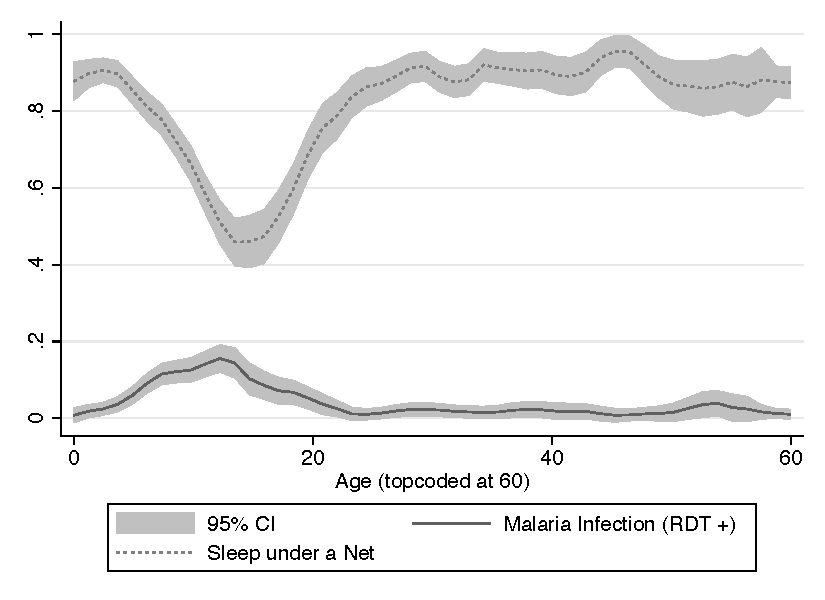
\includegraphics[scale=0.7]{dips.pdf}
\caption{Malaria Infection and Mosquito Net Usage}
\label{dips}
\floatfoot{\textit{Notes:} The two lines show the relationships between malaria infection (mosquito net usage) and age in our baseline survey respectively based on local polynomial regressions. We collect the data of mosquito net usage and malaria infection by household survey and rapid diagnosis test (RDT). See \autoref{sec:data} for the details.}
\end{figure}

% We find that, for each additional year of schooling, a perfectly targeted distribution is USD 288.76--290.07 (or 96.9--97.3\%) cheaper than a universal distribution if we assume no targeting costs exist. These findings provide important insights for understanding basic income programs \citep{ravallion_vox,hanna_universal_2018,banerjee_universal_2019}: although the free distribution of nets will facilitate human capital investment, distributing nets to everyone will not be efficient.


% Yet, to the best of our knowledge, no study investigated the role of decisions within family 

% In the last one decade, the governments and international organizations have promoted free distribution of LLINs to achieve universal coverage. actual usage of nets is left with decisions within each family. 

% . The government often targets pregnant women or children under five years as the most vulnerable from malaria and provides such information to households.  Also, school-aged children may often sleep separately from their parents, which might need more nets to allocate the nets to them than to infants. 

% We investigate two questions regarding the above issues of school-aged children in this study. First, we study the effect of using nets on their school attendance. Our hypothesis is that because using nets will prevent malaria infection and thus reduce absence due to sickness.  Attendance in schools will facilitate human capital accumulation and affect their economic outcomes in the long-run. Second, we study the cost-effectiveness of using or distributing nets to increase years of schooling. We first discuss the cost-effectiveness of using nets. Then, we discuss the cost-effectiveness of universal coverage, distributing nets to all the households for free. By universal coverage, nets will reach to non-users, but it might induce inclusion error such as distributing HHs who already have enough number of nets or will allocate received nets to other members. We compare it with an alternative and feasbile strategy, an age-based targeting where we distribute nets only for households who have pupils.  


Our research design exploits a natural experimental situation in Madagascar. In 2009, the Malagasy government introduced the free distribution of LLINs. Because of limited capacity, it distributed nets on different dates for different regions. To exploit this different distribution timing, we conducted our survey in the area around the border of two regions three times: before the first distribution, after the first distribution, and after both regions had received the nets. In these surveys, we collected household-level information about mosquito net usage and school attendance. We also gathered school attendance records from local schools. Furthermore, we examined the malaria infections among all the villagers by using a rapid diagnosis test (RDT).


Obtained by combining these data from households, schools, and health inspections, our main empirical results show that the distribution of LLINs significantly reduced school absences. This schooling effect seems to be caused by the increase in the use of LLINs and the decrease in the number of malaria infections. On average, using LLINs significantly reduced school absences among children aged 6--12 by approximately 19 days per year. On the contrary, we find no influence on school enrollment, adult malaria infection, or household income. An LLIN costs only USD 11.12--13.49 for each additional year of schooling, suggesting that LLINs, which have been recognized as a core preventive tool to tackle malaria infection, are also a cost-effective measure for enhancing school attendance rates. We also find that universal coverage costs USD 630.22 for an additional year of schooling owing to the large inefficiencies associated with substantial inclusion errors. To reduce these, we propose a feasible and simple targeting strategy: excluding households without any members aged 6--12. A net distribution with this strategy is estimated to only cost USD 273.57 for an additional year of schooling. 


% This study contributes to four strands of the literature.  First, this study contributes to the literature on the social impacts of health interventions in developing countries. Previous studies investigate the impact of various health interventions such as deworming \citep{miguel_worms:_2004}, medical care for very low birth weight \citep{}(Bharadwaj et al. 2013), HIV information \citep{dupas_teenagers_2011,duflo_education_2015}  or malaria eradication programs such as DDT spraying \citep{lucas_economic_2005,bleakley_malaria_2010,lucas_malaria_2010,cutler_early-life_2010,venkataramani_early_2012,barofsky_malaria_2015}.
% Along similar lines, we contribute to the literature by studying the impact of LLINs on school attendance, overlooked intervention and economic outcome in the literature. 

% Second, we contribute to the growing literature of LLINs by focusing on its impact on pupils, under-investigated sample in the literature, and targeting issues. Existing studies on LLINs have focused on LLIN adoption decisions such as how the types of distribution or subsidies affect their adoption or intra-household allocation \citep{blackburn_bednets_2008,hoffmann_intrahousehold_2009,cohen_free_2010,tarozzi_micro-loans_2014,dupas_short-run_2014}.\footnote{\cite{cohen_free_2010} examine the free distribution and cost-sharing in terms of demand and usage rates. \cite{tarozzi_micro-loans_2014} conduct a randomized controlled trial to compare the impact of a free distribution of mosquito nets to that of  loans for nets, finding that free distribution increases the usage rates of mosquito nets more than loans do. 
% \cite{dupas_short-run_2014} examines whether short-run subsidies can lead to long-run adoption and discovers a learning effect, but no anchoring effect. \cite{blackburn_bednets_2008} analyze purchasing behaviors by adopting a structural estimation in a static, discrete-choice framework.
% \cite{hoffmann_intrahousehold_2009} studies the intra-household allocation of mosquito nets.}  We complement the literature by looking at 

% Third,  this study contributes to the research on anti-poverty targeting programs. A large portion of the literature studies the efficacy of targeting methods in developing countries, such as proxy means tests, self-targeting, geographic targeting, and community targeting in developing countries \citep{nichols_targeting_1982,coady_targeting_2004,elbers_poverty_2007,ravallion_how_2009,alatas_targeting_2012,brown_poor_2016}. Unlike these studies, we calculate the cost of universal coverage by comparing the cost of a perfectly targeted LLIN distribution to children aged 6--12
% to that of a universal distribution. We find that, for each additional year of schooling, a perfectly targeted distribution is USD 288.76--290.07 (or 96.9--97.3\%) cheaper than a universal distribution if we assume no targeting costs exist. These findings provide important insights for understanding basic income programs \citep{ravallion_vox,hanna_universal_2018,banerjee_universal_2019}: although the free distribution of nets will facilitate human capital investment, distributing nets to everyone will not be efficient.


% Fourth, our study is broadly linked with the literature on disease and development. The effect of other diseases such as influenza, trypanosomiasis,  are also investigated \citep{acemoglu_colonial_2001,almond_is_2006,alsan_effect_2015}. We contribute to this literature by adding additional evidence of the negative impact of malaria.


The rest of the article is organized as follows: Section \ref{sec:data} explains the data and provides descriptive statistics.
Section \ref{Feb 02 20:20:28 2013} shows
the empirical results, followed by concluding remarks in Section 4.

\section{Data and Descriptive Statistics}

\label{sec:data} 
\subsection{Data}

% % Malagasy government planned the nation-wide
% free distribution campaign of LLINs in 2009--2010, because of increasing
% malaria infection rate. As ascertained from our interview of the government officials, they
% planned to distribute one net per three household members for each household
% because usually, up to three people can sleep in one net. Hence, the
% government provided one net to a three-member household, and two nets to a
% four-member household.

% However, because of their logistical capacity constraint, the government could not
% distribute nets across the whole country at the same time. The government
% divided the country into several parts, and prioritized the distribution on
% the basis of malaria incidence rate. 


We conducted our survey in an area where malaria is prevalent, namely the border area between the Atsinanana and Analanjirofo regions along the east coast of Madagascar (\autoref{map}). There is distinct seasonality in this area: the wet season runs from December to May and the dry season from June to November. In the southern boundary area, Atsinanana, LLINs were distributed in December 2009. In the Analanjirofo region, located north of the boundary, LLINs were provided in June 2010. Based on this six-month gap in the distribution of nets, we label Atsinanana the treated group and Analanjirofo the control group. Figure %
\ref{map} shows the location of our survey respondents: villages 1--12 are located in the Analanjirofo region and
villages 13--18 are in the Atsinanana region. Our research strategy is to exploit this exogenous
variation in the timing of the free distributions. Household surveys were conducted exclusively for our study by the Institut
National de la Statistique de Madagascar (INSTAT) three times. We thus obtained panel data for a first wave (baseline; dry season), second wave (midline; rainy season), and third wave (endline; dry season) (\autoref%
{f:timing}).\footnote{Although women who go to the CSB (public medical center) for
childbirth can obtain nets there, during the free distribution,
there was no other way to receive nets for free. People in both areas can buy mosquito nets from NGOs for 3000 Ariary.}

In the survey, we collected basic information on each household member, such as age,
education level, malaria infection history, and mosquito net usage as well as household information such as income and assets. For children, we also asked about the number of days they were absent from school.\footnote{%
In the first wave, we only asked this question in reference to the previous month. In the
second and third waves, we asked the same question in reference to  the six months since the previous wave.}
Although we gathered information on all household members, we focused on primary school-aged children (i.e., 6--12 years old).


To detect malaria infection,\footnote{%
Detecting symptoms such as anemia \citep{cohen_free_2010} or using a hemoglobin test \citep
{blackburn_bednets_2008} can be used as a proxy.} we employed a validated RDT
(Carestart\textregistered, by Access Bio).\footnote{This test has over 90\% sensitivity (i.e., 1 minus the type I error probability) and
specificity (i.e., 1 minus the type II error probability) for detecting a malaria infection.}\footnote{Because the data in the first wave do not distinguish among the different types of malaria, ``malaria positive,'' as used in this
study, includes all four types of \textit{Plasmodium} species in addition to 
\textit{Plasmodium falciparum} (pf), the most serious one. 
Of the 272 malaria-positive cases in the second wave, 179 are pf positive, 81 are mixed positive, and 12 are non-pf positive.} If a person was detected to be malaria
positive, we provided an ACT drug that treats malaria (Coarsucam \textregistered). Thus, if a person was
found to be infected by malaria in the second (third) survey, we can assume that he or she was infected for the first time between the first and second (second and third) surveys.



\begin{figure}[h]
\centering
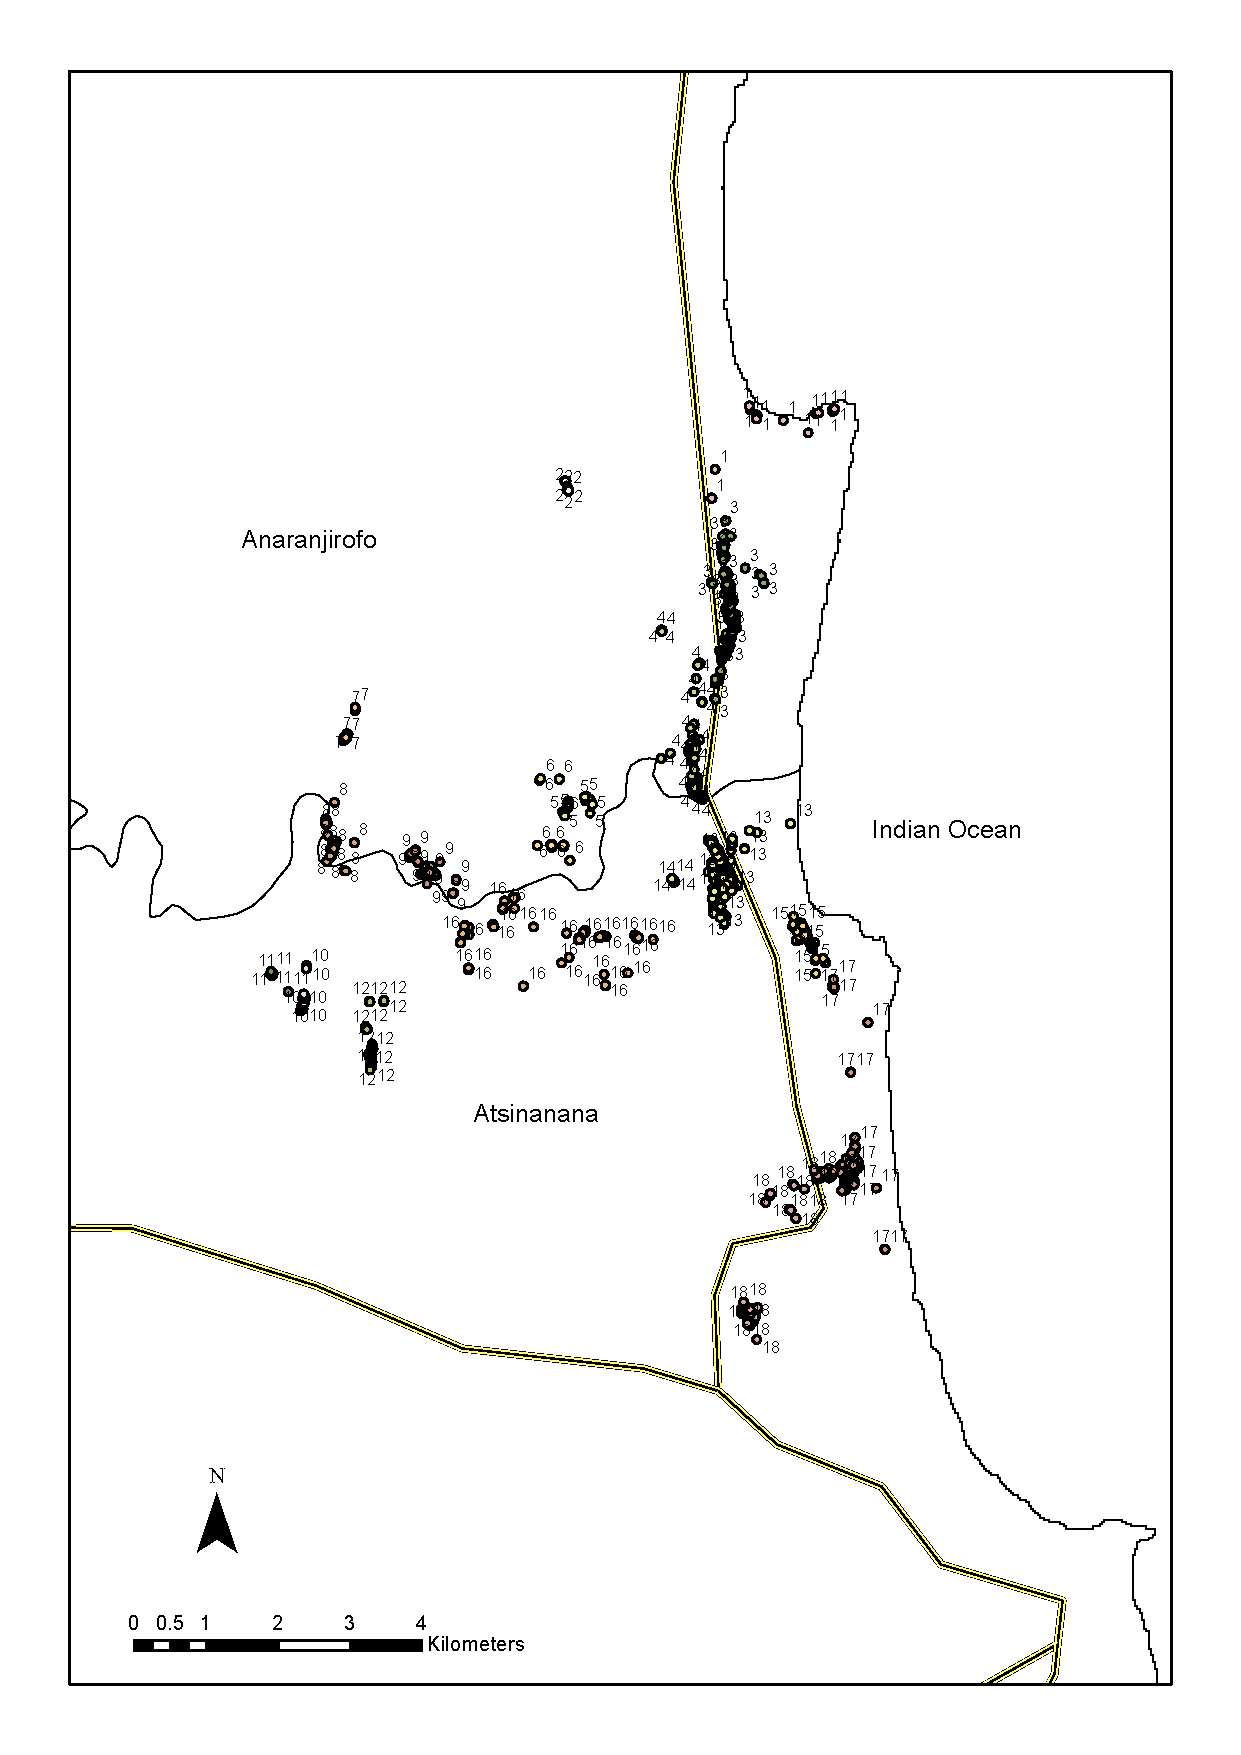
\includegraphics[scale=0.7]{madagascarmap.pdf}
\caption{Map of Households and Villages}
\label{map}
\floatfoot{\textit{Notes:} Yellow lines show main roads, the black line in the middle shows the boundary between the two provinces. Circles show households in our sample and the numbers above the circles indiate the villages.}
\end{figure}

\begin{table}[h]
\caption{Data Collection and Free Distribution}
\label{f:timing}\centering
\begin{tabular}{c c c c c c} 
 &&&\\
 &Dry season&\multicolumn{2}{c}{Wet season}&\multicolumn{2}{c}{Dry season}\\ \cmidrule(lr){2-2}\cmidrule(lr){3-4}\cmidrule(lr){5-6} 
 &Dec. 2009& Dec. 2009-Jan. 2010& May 2010 & June 2010 & Dec. 2010 \\ [0.5em]\hline 
 Atsinanana Region&  First Wave& Free Distribution &  Second Wave & & Third Wave\\ [0.5em]
 Analanjirofo Region& First Wave& &  Second Wave & Free Distribution &Third Wave \\
\end{tabular}
\end{table}


\subsection{Baseline Balance and Attrition}

\label{Feb 02 20:20:11 2013}


We performed baseline balancing tests by comparing the treatment group (South) to the control group (North).
Panel A in \autoref{descriptive_merge_child} shows the comparison of children aged 6--12 in these two regions using our survey data. In the control region, the malaria infection rate is higher and the mosquito net usage rate is lower. In particular, all the high malaria risk villages are in the control group. Based on a regression of the treatment group dummy on a set of these observables, treatment status is orthogonal to the observables conditional on malaria risk. Panel B in \autoref{descriptive_merge_child} displays the
household-level variables: number of nets owned, household
size, number of members who sleep under nets, household
knowledge about the effectiveness of mosquito nets for malaria prevention, and
altitude.\footnote{\cite{bodker_relationship_2003} show that altitude influences the risk of contracting malaria, but all households in our
study were located below an altitude of 100 meters, which is a much lower variation than that considered by \cite{bodker_relationship_2003}.} Except for the number
of nets and altitude, these variables were well-balanced. According to a joint test, the orthogonality of treatment status is not necessarily rejected. In any case, to cope with the potential bias arising from baseline imbalance, we controlled for the dummies representing the high malaria risk village, adding their interaction terms with the wave fixed effects.\footnote{See the Appendix for the results when controlling for the other village-level variables.} To examine the pre-trend, we visited two local clinics on the main road to obtain the date of the malaria infection patterns before the LLIN distribution. \autoref{cbsmalariacase} shows that the two regions exhibit largely similar trends, supporting the parallel trend assumption.
% use "/Users/j_yamasaki/Yamasaki_Lab Dropbox/YAMASAKI Junichi/Madagascar_LLIN/presentation and draft/cbsmalaria.dta" 
% tsline rdt_f rdt_m,ytitle("Malaria Cases") legend(label(1 "Foulpointe (South)") label(2 "Mahambo (North)")) xlabel(576 582 588 594,valuelabel) recast(connected)
% graph export cbsmalariacase.pdf,replace
\begin{figure}
\centering
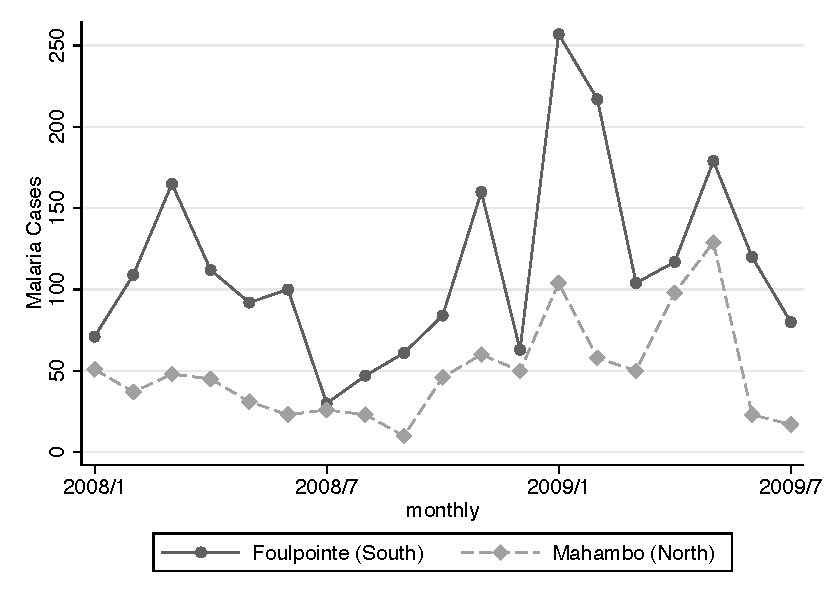
\includegraphics[scale=1]{cbsmalariacase.pdf}
\caption{Malaria Cases in Local Clinics}
\label{cbsmalariacase}
\floatfoot{\textit{Notes:} This graph shows the malaria cases in clinics in Foulpointe and Mahambo respectively. }
\end{figure}




\begin{table}[h]
\caption{Descriptive Statistics}

\begin{adjustbox}{max width=\textwidth}
\begin{threeparttable}
\label{descriptive_merge_child}\centering
% descriptive_children
% descriptiveh
\begin{tablenotes}
\item The standard errors are the 18 village-level cluster-robust standard errors in Panels A and B and the 31 grade * school-level cluster-robust standard errors in Panels C and D.  \sym{+} \(p<.10\), \sym{*} \(p<.05\), \sym{**} \(p<.01\), and \sym{***} \(p<.001\)
\end{tablenotes}
\end{threeparttable}
\end{adjustbox}
\end{table}




% \begin{table}[h]
% \caption{Descriptive Statistics (Seaside)}\centering
% \input{descriptiveb}
% \end{table}

% \begin{table}[h]
% \caption{Descriptive Statistics (Children)}
% \label{Feb 04 00:35:04 2013}\centering
% \input{descriptive_cmerge}
% \end{table}

% \begin{table}[h]
% \caption{Descriptive Statistics (Children, Seaside)}
% \label{Feb 04 00:35:09 2013}\centering
% {
\def\sym#1{\ifmmode^{#1}\else\(^{#1}\)\fi}
\begin{tabular}{l*{1}{cccccc}}
\hline\hline
                    &\multicolumn{6}{c}{}                                                         \\
                    &   Untreated&     Treated&        Diff&        s.e.& Untreated N&   Treated N\\
\hline
RDT +               &    .1002278&    .0639269&    .0363008&    .0185199&         439&         438\\
Sleep in a Net      &    .6219239&    .6748879&    -.052964&     .031943&         447&         446\\
Absence  Last Month &    1.181495&    1.152174&    .0293207&    .2789071&         281&         276\\
Sick Absence Last Month&    .5907473&     .692029&   -.1012817&    .1543376&         281&         276\\
\hline
Observations        &         893&            &            &            &            &            \\
\hline\hline
\end{tabular}
}

% \end{table}

% \begin{table}[h]
% \caption{Descriptive Statistics (Household)}
% \label{Feb 09 21:19:54 2013}\centering
% 

N. of Possesed Net  &    1.338594&     1.53484&    -.196246&    .0458328&         697&         531\\
HH Size             &    3.466284&    3.551789&    -.085505&     .106751&         697&         531\\
Members Using Net   &    2.647059&    2.708098&   -.0610391&    .0941437&         697&         531\\
Knowledge of Usefulness&    .7099494&    .6795132&    .0304362&    .0280425&         593&         493\\
Altitude            &    57.01722&    19.25424&    37.76298&     23.1725&         697&         531\\

Observations        &        1228&            &            &            &            &            \\


% \end{table}

% \begin{table}[h]
% \caption{Descriptive Statistics (Household, Seaside)}
% \label{Feb 09 21:20:00 2013}\centering
% 

N. of Possesed Net  &    1.334661&     1.53484&   -.2001786&     .050552&         502&         531\\
HH Size             &    3.428287&    3.551789&   -.1235022&    .1139788&         502&         531\\
Members Using Net   &    2.611554&    2.708098&   -.0965441&    .1027539&         502&         531\\
Knowledge of Usefulness&    .7356828&    .6795132&    .0561696&    .0295966&         454&         493\\
Altitude            &     44.0259&    19.25424&    24.77166&    19.32863&         502&         531\\

Observations        &        1033&            &            &            &            &            \\


% \end{table}

To check the systematic attrition of the panel, we regressed a dummy variable, which takes the value of one if a household has dropped from the panel and zero otherwise, on a set of observed variables such as the RDT-positive dummy. We found no correlation between the attrition dummy variable and key explanatory
Variables, except household size, which showed a weak correlation.\footnote{See \autoref{drop_2nd3rd_child} for the results.} However, if a household member was
absent, we could not collect data on malaria infection by using the RDT. Nonetheless, the proportion of unavailable RDT cases was very low, approximately 3.2\%.

\subsection{School Attendance Record}

% Other than the household data noted above, we also collected attendance record sheets from
% primary schools in this region to obtain additional data about schooling for robustness checks. The sheets include whether each
% student was present or absent, or the day was holiday. The book is
% recorded manually, so INSTAT staff digitalized them. Unfortunately, the list
% of names were not to able to be digitalized because of bad handwriting and
% missing names, so we could not match this data with our household-individual
% level data. However, it is still useful to compare the effect of the
% distribution from two distinct data source to check them reconcilable.

Panels C and D in \autoref{descriptive_merge_child} show the descriptive statistics for the data from the school attendance records. To examine  school absences and the absence rate, Panel C compares the January 2009 data to the June 2009 data.\footnote{The absence rate is adjusted for holidays and school closures.} Neither of these variables shows significant differences between the two regions. Panel D presents the comparison for June 2009 and December 2009, which corresponds to the first wave, showing nonsignificant differences. The histogram of the number of absence days during the first wave also confirms a baseline balance (\autoref{f:schoolabsence_balance}).

The number of absence days is smaller in the school record data than that in our household survey: attendance books record fewer than one absence day per month, whereas the survey data report more than one absence day per month. This discrepancy may be attributed to the nature of each dataset. Although absences in the household survey included cases where the teacher was absent, the school attendance sheet recorded teacher absences as holidays. However, absences due to sickness are captured well in both datasets.


% Schools are basically closed from July to September because of summer vacation. Therefore, we don't have any attendance book for August, and only a few data is available for July in 2009 and  September in 2008 since some schools have slightly different calender.

% \begin{table}[h]
% \caption{Descriptive Statistics (From The Attendance Book)}
% \label{t:descriptiveattendance}\centering
% % \input{descriptiveattendance_merged}
% \begin{threeparttable}
% \begin{tabular}{l*{1}{cccccc}}
% \hline\hline
%                                                                             \\
%                     &   Control&     Treated&        Diff&        s.e.&Control region N&Treated region N\\
%               \multicolumn{6}{l}{{\it Panel A: 1st Phase (June/2009 -- Dec/2009)}  } \\

% \hline
% Absence per Month   &    .2286567&     .235363&   -.0067063&    .0684679  &        1675&        1708\\
% Absence Rate              &    .0160048&    .0185812&   -.0025764&    .0061079&        1481&        1611\\
% \hline
% \\

% % \multicolumn{6}{l}{{\it Panel B: Seaside Sample, Oct/2009 -- Dec/2009}  } \\
% % \hline
% % Absence   &    1.140794&    .5470085&    .5937857\sym{+}&    .3147847&         277&         234\\
% % Absence Ratio &    .0249692&    .0110082&     .013961\sym{+}&    .0066564&         277&         234\\
% % Absence (1 month)     &    .5884477&    .1923077&      .39614\sym{+}&     .2052406&         277&         234\\
% % Absence Ratio (1 month)&    .0294794&    .0096266&    .0198528\sym{+}&    .0102448 &         277&         234\\
% % Observations        &         511&            &            &            &            &            \\
% % \\

% \multicolumn{6}{l}{{\it Panel B:  Pre-1st Phase (Jan/2009 - June/2009) }  } \\
% \hline
% Absence per Month   &    .3898121&    .2977575&    .0920547&    .1166387 &        2768&        2408\\
% Absence Rate          &    .0253459&    .0085371&    .0021898&    .0024031&        2343&        2032\\
% \hline \hline
% % \multicolumn{6}{l}{{\it Panel D: Seaside Sample,  Sep/2008 -- Oct/2009}  } \\
% % \hline
% % Absence   &    4.732194&     2.68018&    2.052014\sym{+}&     .8965615&         351&         222\\
% % Absence Ratio &    .0295039&    .0174536&    .0120503&    .0063282&         351&         222\\
% % Observations        &         573&            &            &            &            &            \\
% % \hline\hline
% \end{tabular}
% \begin{tablenotes}
% \item  standard errors are 31 Grade * School-level cluster robust.  \sym{+} \(p<.10\), \sym{*} \(p<.05\), \sym{**} \(p<.01\), \sym{***} \(p<.001\)
% \end{tablenotes}
% \end{threeparttable}
% \end{table}




% \begin{figure}[h]
% \centering
% 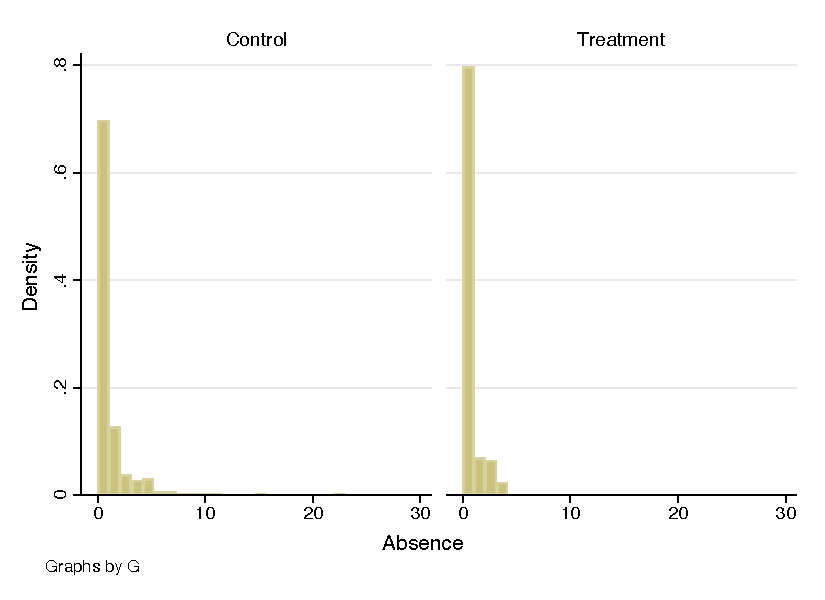
\includegraphics[scale=0.8]{schoolabsence_balance_b.pdf}
% \caption{The Distribution of Absent Days in the 1st wave (From The Attendance Book, Seaside Sample)}
% \label{f:schoolabsence_balance_b}
% \end{figure}


% \begin{table}[h]
% \caption{Descriptive Statistics (From The Attendance Book, Seaside)}
% \label{Feb 12 13:01:00 2013}\centering
% {
\def\sym#1{\ifmmode^{#1}\else\(^{#1}\)\fi}
\begin{tabular}{l*{1}{cccccc}}
\hline\hline
                    &\multicolumn{6}{c}{}                                                         \\
                    &   Untreated&     Treated&        Diff&        s.e.&Untreated region N&Treated region N\\
\hline
Absence 1 month     &    .5884477&    .1923077&      .39614&    .0976321&         277&         234\\
Absence Ratio       &    .0294794&    .0096266&    .0198528&    .0048839&         277&         234\\
\hline
Observations        &         511&            &            &            &            &            \\
\hline\hline
\end{tabular}
}

% \end{table}

% \begin{table}[h]
% \caption{Descriptive Statistics (From The Attendance Book, One Year Before)}
% \label{t:descriptiveattendance 2}\centering
% \input{descriptiveattendancewave0}
% \end{table}

% \begin{table}[h]
% \caption{Descriptive Statistics (From The Attendance Book, One Year Before,
% Seaside)}
% \label{Feb 12 13:01:00 2013 2}\centering
% \input{descriptiveattendancewave0_b}
% \end{table}


\section{Empirical Results}

\label{Feb 02 20:20:28 2013}

\subsection{Effect of Free LLIN Distribution on Schooling}

To investigate the impact of the free distribution of LLINs on school absences, we postulate
the following econometric model: 
\begin{gather}
\text{Absence}_{it}=\alpha _0+\alpha _1 \text{
Distributed} _{it} + \text{Individual Fixed Effects}_i + \text{Wave Fixed Effects}_t +  \epsilon _{it}
\end{gather}
where $\text{Absence}_{it}$ is the number of absence days due to sickness in the past six months, $\text{Distributed%
} _{it}$ is an indicator variable that takes the value of one if an LLIN has been freely distributed and zero otherwise, and $\epsilon _{it}$
is the error term.\footnote{Because, in the first
wave, we did not ask in our survey about absence days in the previous six months,
we only employ the second and third wave data to estimate this model.}

\autoref{t:absence3rd_questionnaire_child} shows the estimation results based on our survey data; LLIN distribution decreased the number of absence days from school by 1.36 days per six months (see column (1)). The result is robust even after controlling for the village-level average number of absence days in the first wave (column (2)) as well as the time-variant effect of the high malaria risk dummy that takes the value of one if a village's malaria infection rate in the first wave exceeded 10\% (column (3)). In columns (4)--(6), we employ school enrollment as an outcome variable. The point estimate of the treatment effect is not statistically significant in all the specifications. Since we have only 18 villages, the cluster-robust standard errors might over-reject the null hypothesis---even when using the finite sample adjustment. Following \cite{cameron_bootstrap-based_2008}, we also show the p-value for testing the null hypothesis that the treatment variable has no effect, using the wild bootstrap method, but the qualitative results remain the same regardless of the standard errors used.\footnote{In \autoref{t:absence3rd_questionnaire_child_app}, we also control for the variables that did not pass the baseline balancing tests, but the result is unchanged.} 

As an additional robustness check, especially against any possible recall errors, we analyze the school attendance book data.\footnote{Primary school students are mainly 6--12 years old.
% Because we are not able to match this data with
% our questionnaire, and attendance book does not contain students' ages, we
% simply use all samples in the attendance book data.
\autoref{t:ageandclass_2nd} shows the relationships between age and grade
in the second wave of survey data.} By using the number of absence days per month as the outcome variable, we estimate equation (1). 
\autoref{t:olsabsence_dailyattend_monthly_withtrend_child} summarizes the results for absence days.\footnote{\autoref{t:olsabsence_dailyattend_monthly_withtrend_child_app} shows the results using the monthly absence rate as the outcome variable.} In addition to the school fixed effects and the wave effects, we consider seasonal fixed effects, a school-level trend, and school-level seasonal fixed effects.
% a  similar regression model with the column (1) of Panel A in \autoref{t:olsabsence_dailyattend_monthly_withtrend_child} in column (1) and for robustness check, in other columns we added seasonal fixed effects,  school specific linear trend or school specific seasonal fixed effects by including data before 09/Jul. 
The average effect of LLIN use on absence days ranges from -0.116 to -0.191 days per month, which corresponds to -0.696 to -1.146 days per six months. These numbers are largely consistent with the point estimates we obtained from the survey data reported in \autoref{t:absence3rd_questionnaire_child}. 
% Note that absence due to sick in the questionnaire will be comparable with absence in attendance sheet, because in attendance sheet teacher's absence, the major reason in the absence in the questionnaire, will be not recorded as absence. 
 

% \footnote{A small fraction of the sample  dropped because of teacher's absence over the period and absence ratio (absence days over school open days) cannot be defined.} 

\begin{table}[h]
\caption{Effect of Net Distribution on Schooling (Based on the Survey Data)}
\label{t:absence3rd_questionnaire_child}\centering
\begin{adjustbox}{max width=\textwidth}
\begin{threeparttable}
\begin{tabular}{l*{7}{c}}
\hline\hline
          &\multicolumn{3}{c}{Sick Absence (6 Months)}&\multicolumn{3}{c}{Enrollment}\\   \cmidrule(lr){2-4} \cmidrule(lr){5-7}
                          &\multicolumn{1}{c}{(1)}&\multicolumn{1}{c}{(2)}&\multicolumn{1}{c}{(3)}&\multicolumn{1}{c}{(4)}&\multicolumn{1}{c}{(5)}&\multicolumn{1}{c}{(6)}\\

\hline
Distributed         &         -1.362\sym{*}  &      -1.363\sym{*}  &      -1.204\sym{*}      &          -0.0384         &     -0.0311         &     -0.0305 \\
                   &     (0.602)         &     (0.576)         &     (0.468)                 &     (0.0222)         &    (0.0238)         &    (0.0244)         \\

Individual Fixed Effects and Wave Fixed Effects &         Yes         &         Yes         &         Yes         &         Yes         &         Yes         &         Yes         \\

Pre-village-level Absence * Wave Fixed Effects&          No         &         Yes         &         Yes         &          No         &         No         &         No         \\

Pre-village-level Enrollment * Wave Fixed Effects&       No         &          No     & No&     No         &         Yes         &         Yes         \\

Pre-high Malaria Risk Village * Wave Fixed Effects&          No         &          No         &         Yes         &          No         &          No         &         Yes         \\
\hline
p-value             &       0.038         &       0.031         &       0.020         &       0.102         &       0.209         &       0.229         \\
Wild Bootstrap p-value &       0.045         &       0.043         &       0.062         &       0.064         &       0.220         &       0.259         \\
Number of Observations        &        1122         &        1122         &        1122         &      2147         &        2147         &        2147         \\
% \\
%                       &\multicolumn{3}{c}{Enrollment} &&& \\  \cmidrule(lr){2-4} 
                    
%         \textit{Panel B: Enrollment}                   &\multicolumn{1}{c}{(1)}&\multicolumn{1}{c}{(2)}&\multicolumn{1}{c}{(3)} &&& \\
% \hline
% Distributed         &     -0.0384         &     -0.0311         &     -0.0305         \\
%                     &    (0.0222)         &    (0.0238)         &    (0.0244)         \\
% 
% Individual Fixed Effects and Wave Fixed Effects &         Yes         &         Yes         &         Yes        &&& \\
% 
% Pre-village-level Enrollment * Wave Fixed Effects&          No         &         Yes         &         Yes        &&& \\
% 
% Pre-high Malaria Risk Village * Wave Fixed Effects&          No         &          No         &         Yes        &&& \\
% \hline
% Observations        &        2147         &        2147         &        2147        &&& \\
\hline\hline
\end{tabular}
\begin{tablenotes}
\item Cluster-robust standard errors (18 village-level with a finite sample adjustment) are in parentheses. \sym{+} \(p<.10\), \sym{*} \(p<.05\), \sym{**} \(p<.01\), and \sym{***} \(p<.001\). In columns (1)--(3), we only use the second and third waves because we obtain data on the outcome variable after the first wave. In columns (4)--(6), we use all the waves. The \textit{p-value} and \textit{Wild Bootstrap p-value} are used to test whether the treatment coefficient is zero, using the standard error in the table and the  cluster-robust wild bootstrap, respectively.
\end{tablenotes}
\end{threeparttable}
 \end{adjustbox}
\end{table}
% \begin{table}[h]
% \caption{The Effect of Distribution on Absent Days Because of Sick (From the
% Questionnaire)}
% \label{Feb 05 17:50:55 2013}\centering
% {
\def\sym#1{\ifmmode^{#1}\else\(^{#1}\)\fi}
\begin{tabular}{l*{4}{c}}
\hline\hline
                    &\multicolumn{1}{c}{(1)}&\multicolumn{1}{c}{(2)}&\multicolumn{1}{c}{(3)}&\multicolumn{1}{c}{(4)}\\
                    &\multicolumn{1}{c}{Age 6--12}&\multicolumn{1}{c}{Age 13--19}&\multicolumn{1}{c}{Age 6--12}&\multicolumn{1}{c}{Age 13--19}\\
\hline
Distributed         &      -1.517\sym{*}  &      -0.828         &      -1.371\sym{**} &      -0.683         \\
                    &     (0.533)         &     (1.273)         &     (0.368)         &     (1.229)         \\
[1em]
Constant            &       2.117\sym{***}&       2.220\sym{*}  &       1.971\sym{***}&       2.074\sym{*}  \\
                    &     (0.501)         &     (0.932)         &     (0.319)         &     (0.855)         \\
\hline
Observations        &         573         &          64         &         470         &          50         \\
\hline\hline
\multicolumn{5}{l}{\footnotesize Standard errors in parentheses}\\
\multicolumn{5}{l}{\footnotesize Column 3 and 4 use only seaside samples. Cluster robust SEs (village level).}\\
\multicolumn{5}{l}{\footnotesize Odd colums are 6--12, and even colums are 13--19-years-old samples.}\\
\multicolumn{5}{l}{\footnotesize \sym{*} \(p<0.05\), \sym{**} \(p<0.01\), \sym{***} \(p<0.001\)}\\
\end{tabular}
}

% \end{table}


% \begin{table}[h]
% \caption{The Effect of Distribution on Absent Days (From the Attendance
% Book) }
% \label{Feb 05 17:19:07 2013}\centering
% \input{olsabsence_dailyattend.tex}
% \end{table}
\begin{table}[h]
\caption{Effect of Net Distribution on Absence Days (Based on the School Attendance
Book)}
\label{t:olsabsence_dailyattend_monthly_withtrend_child}\centering
\begin{adjustbox}{max width=\textwidth}
\begin{threeparttable}
\begin{tabular}{l*{5}{c}}
\hline\hline
&\multicolumn{5}{c}{Absence per Month}\\ \cmidrule(lr){2-6}
                    &\multicolumn{1}{c}{(1)}&\multicolumn{1}{c}{(2)}&\multicolumn{1}{c}{(3)}&\multicolumn{1}{c}{(4)}&\multicolumn{1}{c}{(5)}\\\hline
Distributed           &      -0.191\sym{*}  &      -0.167\sym{+}  &      -0.159\sym{+}  &      -0.145\sym{+}  &      -0.116         \\
                    &    (0.0919)         &    (0.0853)         &    (0.0811)         &    (0.0809)         &     (0.115)         \\

School Fixed Effects           &         Yes         &         Yes         &         Yes         &         Yes         &         Yes         \\

Wave Fixed Effects            &         Yes         &         Yes         &         Yes         &         Yes         &         Yes         \\

Season Fixed Effects            &          No         &          No         &         Yes         &         Yes         &          Yes         \\

Linear Trend * School Fixed Effects &          No         &          No         &          No         &         Yes         &          No         \\

Season * School Fixed Effects   &          No         &          No         &          No         &          No         &         Yes         \\
\hline
   p-value&       0.047         &       0.059         &       0.059         &       0.083         &       0.321  \\
Wild Bootstrap p-value &       0.082         &       0.095         &       0.095         &       0.161         &       0.369         \\
Number of Observations        &       13928         &       19104         &       19104         &       19104         &       19104         \\
\hline\hline
\end{tabular}
\begin{tablenotes}
\item The 31 grade * school-level cluster-robust standard errors are in parentheses. The \textit{p-value} and \textit{Wild Bootstrap p-value} are used to test whether the treatment coefficient is zero, using the standard error in the table and the cluster-robust wild bootstrap, respectively. \sym{+} \(p<.10\), \sym{*} \(p<.05\), \sym{**} \(p<.01\), and \sym{***} \(p<.001\). Column (1) uses only data after June 2009 as was done with the survey data, whereas the other columns include December 2008--June 2009.  \textit{Season Fixed Effects} capture monthly seasonal effects, taking the value of one for January, for example.
\end{tablenotes}
\end{threeparttable}
\end{adjustbox}
\end{table}


% \begin{table}[h]
% \caption{The Effect of Distribution on Absent Probability (From the
% Attendance Book)}
% \label{Feb 06 17:46:20 2013}\centering
% \input{olsabsencep_dailyattend.tex}
% \end{table}

\subsection{Effect of Free Distribution on Mosquito Net Use}

\autoref{f:mqnid} shows the usage rate of
mosquito nets by age based on the 24-hour recall data. We can easily verify that people aged 6--20 did not use
nets in the first wave (panels (C1) and (T1)). However, in the second
wave, most young people in the treated group began to use a
mosquito net (panel (T2)). To capture this more
precisely, we regress the LLIN usage indicator variable on the treatment variable by using the full sample as well as the sample of children aged 6--12. The results reported in Panel A of \autoref{mqnidd3rd_child} confirm that the distribution of free LLINs increased net usage, especially for children aged 6--12.\footnote{See \autoref{mqnidd3rd_child_app} for additional robustness check results.} To explore the reasons behind the lack of mosquito net usage by children aged 6--12, we examine the responses to the subjective questions on mosquito net use conditions. According to the regression analysis, these children are not using nets partially because they sleep on the floor and with fewer parents.\footnote{\autoref{floornetusing} shows the results. Column (1) shows these children's lower usage rate but the coefficient becomes close to zero once we control for a dummy variable indicating whether they sleep on the floor or the number of parents they sleep with in columns (2)--(4). In column (5), we include the interaction terms of these controls with the dummy for children aged 6--12 but we find quantitatively small coefficients for these interactions, which implies that these controls explain well why children aged 6--12 are not using mosquito nets. }\footnote{Another finding in \autoref{f:mqnid} is that the treatment group's usage rate decreased in the third wave, suggesting negative learning effects. We will discuss how this affects our analysis using an instrumental variable (IV) in Subsection \ref{sec:late}.}

In Panel B of \autoref{mqnidd3rd_child} , we only use households that had more than 0.5 nets per member in the first stage. Because typically about two person can share one mosquito net, these households had sufficient number of mosquito nets before the free distribution. As a result, we do not see an economically and statistically significant increase in net usage after the free distribution. 

 % This is natural because kids may not want to sleep with their parents unlike babies, so they tend to sleep alone and sleep on the floor. Then, it would be cumbersome to hang up and down a net every day when they use it on the floor. Also, the campaign by local clinics emphasizing the risk for pregnant women and babies, so nets will be allocated to parents and babies given the size of nets, usually for 2-3 persons. 



%[Intra-household allocation problem.]

\begin{figure}[h]
\centering
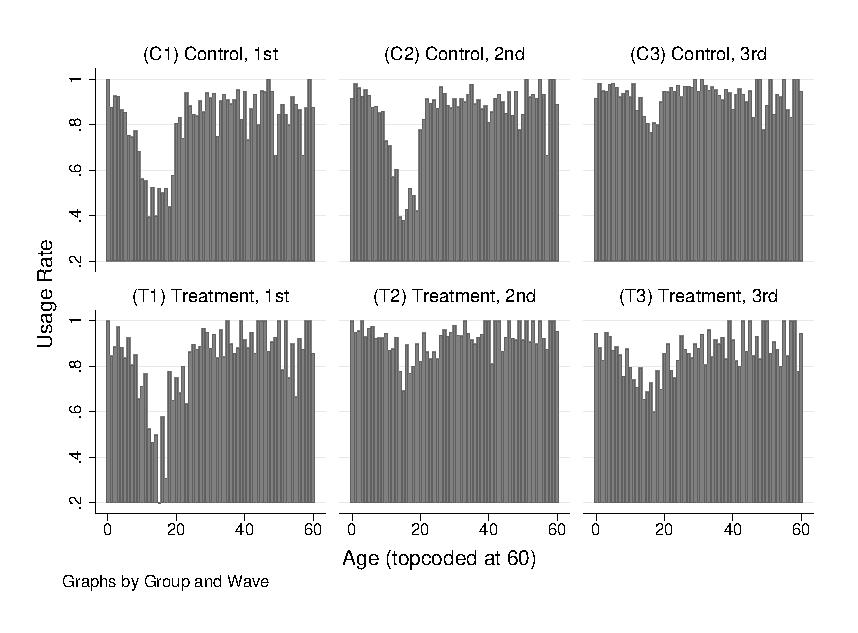
\includegraphics[scale=1]{age60_and_mosquitonet_3rd.eps}
\caption{Age and Net Usage on the Previous Night}
\label{f:mqnid}
\floatfoot{\textit{Notes:} This graph shows the usage rate of mosquito nets in each age, group and wave. Age is topcoded at 60. }
\end{figure}


\begin{table}[h]
\caption{Effect of Net Distribution on the Usage Rate}
\label{mqnidd3rd_child}
\centering
\begin{adjustbox}{max width=\textwidth}
\begin{threeparttable}
\begin{tabular}{l*{4}{c}}
\hline\hline
	&\multicolumn{4}{c}{Sleep under a Net}\\  \cmidrule(lr){2-5}
	&\multicolumn{2}{c}{All Ages}&\multicolumn{2}{c}{6--12 Years Old}\\ \cmidrule(lr){2-3}  \cmidrule(lr){4-5}
                    &\multicolumn{1}{c}{(1)}&\multicolumn{1}{c}{(2)}&\multicolumn{1}{c}{(3)}&\multicolumn{1}{c}{(4)}\\
    \multicolumn{4}{l}{\textit{Panel A: All Households}}  \\ \hline
Distributed         &       0.129\sym{***}&       0.129\sym{***}&       0.154\sym{**} &       0.154\sym{**} \\
                    &    (0.0247)         &    (0.0241)         &    (0.0413)         &    (0.0433)         \\
   \multicolumn{4}{l}{\textit{Panel B: All Households with More than 0.5 Nets per Member in the First Wave}} \\ \hline
Distributed         &      0.0437         &      0.0434         &     -0.0561         &     -0.0515         \\
                    &      (0.0368)         &      (0.0369)         &      (0.0464)         &      (0.0482)         \\


Individual Fixed Effects and Wave Fixed Effects &         Yes         &         Yes         &         Yes         &         Yes         \\

Pre-village-level Net Usage Rate * Wave Fixed Effects&          No         &         Yes         &          No         &         Yes         \\
\hline
p-value in Panel A    &       0.000         &       0.000         &       0.002         &       0.002         \\
Wild Bootstrap p-value  in Panel A &       0.000         &       0.000         &       0.017         &       0.049         \\
Number of Observations   in Panel A        &       11232         &       11232         &        2148         &        2148         \\
Observations in Panel B        &        1671         &        1671         &         181         &         181         \\
\hline\hline
\end{tabular}
\begin{tablenotes}
\item Cluster-robust standard errors (18 village-level with a finite sample adjustment) are in parentheses. In panel A, we use all households, while we only use households that had more than 0.5 nets per member in the first wave per member. For the results in columns (1) and (2) all the samples are used, whereas for those in columns (3) and (4), the 6—12-year-old sample is used. The \textit{p-value} and \textit{Wild Bootstrap p-value} are used to test whether the treatment coefficient is zero, using the standard error in the table and the cluster-robust wild bootstrap, respectively. Data from all the waves are used.
\item \sym{+} \(p<.10\), \sym{*} \(p<.05\), \sym{**} \(p<.01\), and \sym{***} \(p<.001\)
\end{tablenotes}
\end{threeparttable}
\end{adjustbox}
\end{table}
\subsection{Effect of Mosquito Net Usage on the Infection Rate}

To understand the link between mosquito net use and schooling, it
is critical to determine whether using a mosquito net can reduce the malaria infection
rate. First, we adopt the two-stage least squares (2SLS) approach by regressing a binary variable for malaria infection on a binary net-use variable, instrumented by the LLIN treatment variable, using the second wave data. Since these two variables are binary, the estimated coefficient is the local average treatment effect (LATE) of \cite{angrist_two-stage_1995}. As shown in column (1) of \autoref{laterdt_child}, we find a significantly negative coefficient. The result is robust even after additionally controlling for the high malaria risk village dummy (column (2)) and the malaria infection rate at the village level (column (3)).

We also undertake an IV estimation, using the data from all the waves (see columns (4)--(6) in \autoref{laterdt_child}), finding significantly negative treatment effects. Considering that the baseline infection rate is 13\%, the effect size seems to be substantial, ranging from -0.62 to -0.55. Overall, we find that LLIN usage decreased malaria infection almost consistently.\footnote{See \autoref{laterdt_child_app} for additional robustness checks.}



\begin{table}[h]
\caption{Effect of Mosquito Net Use on Malaria Infection}
\label{laterdt_child}\centering
\begin{adjustbox}{max width=\textwidth}
\begin{threeparttable}
\begin{tabular}{l*{6}{c}}
\hline\hline
&\multicolumn{6}{c}{RDT +}\\     \cmidrule(lr){2-7}
                                        &\multicolumn{3}{c}{2SLS (Second Wave)}&\multicolumn{3}{c}{FE-IV (All Waves)}\\  \cmidrule(lr){2-4}  \cmidrule(lr){5-7}

                    &\multicolumn{1}{c}{(1)}&\multicolumn{1}{c}{(2)}&\multicolumn{1}{c}{(3)}&\multicolumn{1}{c}{(4)}&\multicolumn{1}{c}{(5)}&\multicolumn{1}{c}{(6)}\\

\hline
Sleep under a Net      &      -1.094\sym{*}  &      -0.735\sym{**} &      -0.452\sym{**} &      -0.620\sym{*}  &      -0.554\sym{**} &      -0.545\sym{*}  \\
                    &     (0.462)         &     (0.197)         &     (0.148)         &     (0.254)         &     (0.173)         &     (0.220)         \\

Individual Fixed Effects and Wave Fixed Effects &          No         &          No         &          No         &         Yes         &         Yes         &         Yes         \\

Pre-high Malaria Risk Village * Wave Fixed Effects&          No         &         Yes         &         Yes         &          No         &         Yes         &         Yes         \\

Pre-village-level Infection Rate * Wave Fixed Effects&          No         &          No         &          Yes         &          No         &          No         &         Yes         \\
\hline
p-value  &       0.030         &       0.002         &       0.007         &       0.026         &       0.005         &       0.024          \\
Wild Bootstrap p-value &       0.008         &       0.004         &       0.036         &       0.014         &       0.017         &       0.065     \\
Number of Observations        &         696         &         696         &         696         &        2043         &        2043         &        2043         \\
\hline\hline
\end{tabular}
\begin{tablenotes}
\item Cluster-robust standard errors (18 village-level with a finite sample adjustment) are in parentheses. The \textit{p-value} and \textit{Wild Bootstrap p-value} are used to test whether the treatment coefficient is zero, using the standard error in the table and the cluster-robust wild bootstrap, respectively. In columns (1)--(3), we only use the second wave. In columns (4) -- (6), we use all the waves.
\item \sym{+} \(p<.10\), \sym{*} \(p<.05\), \sym{**} \(p<.01\), and \sym{***} \(p<.001\)
\end{tablenotes}
\end{threeparttable}
\end{adjustbox}
\end{table}


\subsection{Effect of Mosquito Net Use or Malaria Infection on Schooling}
\label{sec:late}
We also perform a regression analysis to uncover the effect of mosquito net usage on the number
of absence days. By employing a cross-sectional IV estimation using the second-wave data, we find that using nets decreases sick absences by 11.09--13.45 days in six months (see columns (1)--(3) in \autoref{latemqnabsence62_child}). The effect size corresponds to 2.2--2.67 standard deviations of the sick absence variable in the second wave. To incorporate individual time-invariant heterogeneities, we conduct an FE-IV analysis using the second and third waves (see columns (4)--(6)). The effect size in columns (1)--(3) is larger than that in columns (4)--(6). This difference can be explained by the negative learning effects of net usage: among those who had received nets during the second wave, the proportion of people using nets declined in the third wave (See Section A.1 in the Appendix for the detail). When we only use the sample of those using nets in the third wave, the point estimates approach those reported in columns (1)--(3).\footnote{For example, -5.701 in column (4) becomes -9.70. The other results are available upon request.}

There are two caveats in our results. First, the negative learning effect may be seen as inconsistent with \cite{dupas_short-run_2014}, but the different baseline usage rates can cause this. The shares of household members that slept under a net the previous night in \cite{dupas_getting_2014} and in our data are 0.41 and 0.78, respectively. Therefore, even if we assume the same distribution of learning effects, those who started to use nets in our setting would have systematically weaker learning effects than those in the setting of \cite{dupas_getting_2014}.  Second, even with the negative learning effects due to the high baseline net usage rate, we find that using nets can still generate positive impacts on human capital accumulation. 
% egen test2 = mean(mqnid),by(mhid09 phase)
 % sum test2 if phase==1&hl1==1

To assess the direct effect of malaria infection on absences, we use
the malaria infection variable as an independent variable and distribution as an IV. The
results reported in Panel B of \autoref{latemqnabsence62_child} show that malaria infection increases absence days for children aged 6--12.\footnote{See \autoref{latemqnabsence62_child_app} for additional robustness checks.}

% Also, we show FE-IV analysis in column (4) - (6) and reproduce similar results with column (1) -- (3) unlike in Panel A. This is natural because there will be no seasonality about the impact of infection on absence.\




\begin{table}[h]
\caption{Effect of Mosquito Net Use or Malaria Infection on Schooling}
\label{latemqnabsence62_child}\centering
\begin{adjustbox}{max width=\textwidth}
\begin{threeparttable}
\begin{tabular}{l*{6}{c}}
\hline\hline
                                                                \\
                                                                 &\multicolumn{6}{c}{Sick Absences (6 months)}\\  \cmidrule(lr){2-7}

                                       &\multicolumn{3}{c}{2SLS (Second Wave)}&\multicolumn{3}{c}{FE-IV (Second \& Third Waves)}\\  \cmidrule(lr){2-4}  \cmidrule(lr){5-7}
                    &\multicolumn{1}{c}{(1)}&\multicolumn{1}{c}{(2)}&\multicolumn{1}{c}{(3)}&\multicolumn{1}{c}{(4)}&\multicolumn{1}{c}{(5)}&\multicolumn{1}{c}{(6)}\\
                       \multicolumn{6}{l}{\textit{Panel A: Effect of Mosquito Net Use}}\\  \hline

Sleep under a Net      &      -13.45\sym{+}  &      -13.45\sym{+}  &      -11.09\sym{*}  &      -5.701\sym{+}  &      -5.704\sym{+}  &      -5.310\sym{+}  \\
                    &     (7.051)         &     (7.059)         &     (3.941)         &     (2.940)         &     (2.762)         &     (2.523)         \\
                       \multicolumn{6}{l}{\textit{Panel B: Effect of Malaria Infection}}\\  \hline

RDT +               &       11.26\sym{*}  &       11.26\sym{*}  &       15.88\sym{**} &       13.92\sym{+}  &       14.21\sym{+}  &       14.58\sym{+}  \\
                    &     (4.507)         &     (4.519)         &     (4.556)         &     (7.313)         &     (7.230)         &     (8.237)         \\

Individual Fixed Effects and Wave Fixed Effects &          No         &          No         &          No         &         Yes         &         Yes         &         Yes         \\

Pre-village-level Absence * Wave Fixed Effects&          No         &         Yes         &         Yes         &          No         &         Yes         &         Yes         \\

Pre-high Malaria Risk Village * Wave Fixed Effects &          No         &          No         &         Yes         &          No         &          No         &         Yes         \\
\hline
p-value in Panel A            &      0.0745         &      0.0748         &      0.0125         &      0.0704         &      0.0555         &      0.0515      \\
Wild Bootstrap p-value in Panel A&       0.051         &       0.073         &       0.056         &       0.066         &       0.062         &       0.097     \\
Number of Observations in Panel A       &         573         &         573         &      573         &        1122  &    1122         &        1122         \\
p-value  in Panel B &       0.024         &       0.024         &       0.003         &       0.075         &       0.067         &       0.096       \\
Wild Bootstrap p-value  in Panel B            &      0.013         &       0.022         &       0.027         &       0.027         &       0.033         &       0.068         \\
Number of Observations in Panel B       &          563         &         563         &         563         &        1002         &        1002         &        1002            \\
\hline\hline
\end{tabular}
\begin{tablenotes}
\item Cluster-robust standard errors (18 village-level with a finite sample adjustment) are in parentheses. We use distribution as an instrument. The \textit{p-value} and \textit{Wild Bootstrap p-value} are used to test whether the treatment coefficient is zero, using the standard error in the table and the cluster-robust wild bootstrap, respectively. In columns (1)--(3), we only use the second wave. In columns (4)--(6), we use the second and third waves.
\item \sym{+} \(p<.10\), \sym{*} \(p<.05\), \sym{**} \(p<.01\), and \sym{***} \(p<.001\) 
\end{tablenotes}
\end{threeparttable}
\end{adjustbox}
\end{table}


\subsection{Robustness Check}
Since the mosquito nets (Olyset net \textregistered, Sumitomo Chemical) distributed in the campaign
are treated by insecticides, there could be positive externalities of
the treatment across the regional border \citep{hawley_community-wide_2003-1}, potentially causing our treatment effect estimates to be downward biased. According to \cite{gimnig_effect_2003}, an LLIN's externality is valid within
600 meters. The boundary was marked by a river, and the distance between
the households on the different sides of the river was over 600 meters in most 
cases. Hence, in our setting, positive externalities are not necessarily severe. In contrast, another type of externality may exist among the individuals in each household. We thus examine the existence of such externalities based on pre-distribution information, using the following specification:\footnote{%
We also tried to estimate this externality by using the distance from the
border as an instrument for the neighbors' usage rate. However, because the
location of houses does not exhibit a wide distribution, as seen in \autoref{map},
there was insufficient variation in the distance from the border to estimate the effect.}

\begin{gather}
\text{RDT}_{it}=\alpha _0+\alpha _1\text{Distributed} _{it} + \alpha_2 \text{Distributed}_{it} *\text{Non-User Prop in HH}_i \\ \notag \quad \quad + \text{Wave Fixed Effects}_t +\text{Individual Fixed Effects}_t +\text{Wave Fixed Effects}_t*\text{Non-User Prop in HH}_i + \epsilon _{it},
\end{gather}
where $\text{RDT}_{it}$ is the malaria infection dummy and $\text{Non-User Prop in HH}_i$ is a variable defined as the proportion of household members not using nets in the first wave. If there are positive externalities from using nets, the coefficient $\alpha_2$ will be negative; if a respondent is surrounded by non-user household members, the gain from the externalities will be larger. As shown in \autoref{externality_child}, in all specifications, the estimated coefficient, $\alpha_2$, is not statistically significant, lending no support to the existence of positive externalities. In columns (3) and (4), to detect any externalities within each household, we also use another variable, $\text{Infection Rate in HH}_i$, which represents the household-level infection rate during the first wave. The results again do not support the existence of positive externalities.


\begin{table}[h]
\caption{Test of the Externalities of Net Distribution on Malaria Infection (1)}
\label{externality_child}
\centering
\begin{threeparttable}
\begin{tabular}{l*{4}{c}}
\hline\hline                     &\multicolumn{4}{c}{RDT +}\\  \cmidrule(lr){2-5} 
                    &\multicolumn{1}{c}{(1)}&\multicolumn{1}{c}{(2)}&\multicolumn{1}{c}{(3)}&\multicolumn{1}{c}{(4)}\\
\hline
Distributed         &     -0.0724         &     -0.0826         &      -0.109\sym{**} &      -0.102\sym{**} \\
                    &    (0.0513)         &    (0.0492)         &    (0.0332)         &    (0.0306)         \\

Distributed * {Non-User Prop. in Household} &     -0.0436         &     -0.0499         &                     &                     \\
                    &     (0.108)         &     (0.110)         &                     &                     \\
 
Distributed * {Infection Rate in Household} &               &                       &      -0.232         &      -0.198         \\
                    &                     &                     &     (0.285)         &     (0.305)         \\

Individual Fixed Effects and Wave Fixed Effects &         Yes         &         Yes         &         Yes         &         Yes         \\

Pre-village-level Infection Rate * Wave Fixed Effects&          No         &         Yes         &          No         &         Yes         \\

Non-User Prop. in Household or Infection Rate in Household&         Yes         &         Yes         &         Yes         &         Yes         \\ * Wave Fixed Effects&                  &                  &                  &                  \\
\hline
Number of Observations        &        2043         &        2043         &        2043         &        2043         \\
\hline\hline
\end{tabular}
\begin{tablenotes}
\item Cluster-robust standard errors (18 village-level with a finite sample adjustment) are in parentheses. Data from all the waves are used.  \sym{+} \(p<.10\), \sym{*} \(p<.05\), \sym{**} \(p<.01\), and \sym{***} \(p<.001\). 
\end{tablenotes}
\end{threeparttable}
\end{table}

Another way to test the externalities of LLIN through the pesticides is to use an only within-household variation of usage of the mosquito nets to estimate the effect on the malaria infection. Consider the following model for the second period as being the true model:
\begin{gather}
\text{RDT}_{ih}=\beta _0+\beta _1\text{Sleep in a Net} _{ih} + \beta_2 \text{Sleep in a Net}_{h}  + \epsilon _{ih},
\end{gather}
where $\text{Sleep in a Net}_{h}$ is the usage rate of mosquito nets in $i$'s household $h$.

Then, if we estimate the following model using $\text{Distributed}_{ih}$ as an instrument, 
\begin{gather}
\text{RDT}_{ih}=\beta _0+\beta _1\text{Sleep in a Net} _{ih}   + \epsilon _{i},
\end{gather}
the estimated $\beta_1$ (i.e., $\hat{\beta}_1$) might be biased due to omitting $\beta_2 \text{Sleep in a Net}_{h}$, which $\text{Distributed}_{ih}$ also affects.
On the other hand, if we take the within-household difference
\begin{gather}
\text{RDT}_{ih}-\text{RDT}_{jh} =\beta _1(\text{Sleep in a Net} _{ih} - \text{Sleep in a Net} _{jh})     + \epsilon _{ih}-\epsilon _{jh},
\end{gather}
where $j$ refers to the household head in $i$'s household without loss of generality,  we obtain a consistent estimate of $\beta _1$ ($=\tilde{\beta }_1$) by 2SLS. 

If the externalities play a key role in reducing malaria infection, $\hat{\beta}_1$ would be much smaller than $\tilde{\beta}_1$.
\autoref{externality_withinhh2} shows the comparison; the values of $\hat{\beta}_1$ and $\tilde{\beta}_1$ are similar.\footnote{A constant term can be added to the within-household specification when considering different baseline malaria risks between children aged 6--12 and their household head. In column (2), we keep the constant term in the main equation while we use the constant term as an additional instrument in column (3). In columns (4) -- (6), we additionally control for the lag of malaria infection, but the results do not change substantially. } Overall, these two analyses do not support the existence of externalities at the household level.


\begin{table}[h]
\caption{Test of the Externalities of the Distribution on Malaria Infection (2)}
\label{externality_withinhh2}
\centering
\begin{threeparttable}
\begin{tabular}{l*{6}{c}}
\hline\hline

                    &\multicolumn{1}{c}{RDT +}&\multicolumn{2}{c}{$\Delta^{HH}$  RDT+  }&\multicolumn{1}{c}{RDT +}&\multicolumn{2}{c}{$\Delta^{HH}$  RDT+  }\\   \cmidrule(lr){2-2}   \cmidrule(lr){3-4}   \cmidrule(lr){5-5}   \cmidrule(lr){6-7}
                                        &\multicolumn{1}{c}{(1)}&\multicolumn{1}{c}{(2)}&\multicolumn{1}{c}{(3)}&\multicolumn{1}{c}{(4)}&\multicolumn{1}{c}{(5)}&\multicolumn{1}{c}{(6)}\\
\hline
Sleep in a Net      &      -1.094\sym{*}  &                     &                     &      -1.034\sym{*}  &                     &                     \\
                    &     (0.462)         &                     &                     &     (0.392)         &                     &                     \\
[1em]
$\Delta^{HH}$ Sleep in a Net      &                     &      -1.069\sym{**} &      -1.157\sym{***}&                     &      -0.880\sym{**} &      -1.163\sym{***}\\
                    &                     &     (0.339)         &     (0.234)         &                     &     (0.256)         &     (0.274)         \\
Constant            &       1.080\sym{*}  &      0.0110         &                     &       1.038\sym{*}  &      0.0415\sym{***}&                     \\
                    &     (0.413)         &    (0.0165)         &                     &     (0.365)         &   (0.00987)         &                     \\
L.RDT +             &                     No &                     No &                     No &     Yes         &                     No& No                     \\
L.$\Delta^{HH}$  RDT+        &                    No  &                    No  &                    No  &                    No  &      Yes       &      Yes         \\
\hline
Number of Observations        &         696         &         670         &         670         &         663         &         623         &         623         \\
Wild Bootstrap p-value &     0.00400         &           0         &           0         &     0.00600         &     0.00200         &     0.00200         \\
\hline\hline
\end{tabular}
\begin{tablenotes}
\item Cluster-robust standard errors (18 village-level with a finite sample adjustment) are in parentheses. \sym{+} \(p<.10\), \sym{*} \(p<.05\), \sym{**} \(p<.01\), and \sym{***} \(p<.001\). 
\item Column (1) is a copy of column (1) in \autoref{laterdt_child}.
\item We use only the second wave.
\end{tablenotes}
\end{threeparttable}
\end{table}



We also investigate whether bias arises from the potential ``announcement effect,'' namely, that people might have known about the free distribution campaign more than six months in advance and this prevented them from buying nets. This effect would lead to overestimation of the treatment effect of the free distribution on mosquito net usage. In the third wave, we asked respondents whether they knew about the free distribution campaign and its timing beforehand. Only 4\% of households knew about the forthcoming free distribution. However, even without these households with prior knowledge of the free distribution, the estimation results remain the same as the original results (\autoref{distributionknow}). Therefore, any potential bias arising from the announcement effect is not necessarily serious.

To shed light on the direction of the endogeneity, we compare the OLS and IV estimations of the effect of mosquito net use on malaria infection and school absences (\autoref{ivandols}). We find that the OLS coefficients are consistently larger than the IV coefficients, suggesting that the OLS estimates are upward biased.

% On the other hand, column 2 and 4 in the tables show results for 13--19 years old. The estimated results have big standard error so we cannot infer whether OLS is upward or downward biased. We may have to discuss the result by \autoref{ivandolsrdt}  because OLS point estimate is smaller than IV point estimate, which is the opposite from the finding for 6--12 years old. However, because the estimated effect by IV is LATE, so teenagers who starts to use nets because of the distribution might have different effect from other teenagers, in particular, always takers. For example, if teenager compliers do not use nets properly, we may get this pattern. We will discuss this point later again, but the reason of the heterogeneous effect is beyond of the scope of this paper.



We also seek other possible explanations for the net usage effect on school absences. 
An alternative channel is income: net usage by the adult members of a household may increase labor supply and income, thereby raising school attendance rates. This channel may lead to the overestimation of the IV results because the distribution would positively affect the adults' labor supply or income, which is not captured directly in our regression models. To examine this channel, we analyze the impact of the distribution of LLINs on adults' malaria infection and household-level income. We find that net distribution nonsignificant effects on adults' malaria infection (see \autoref{adultrdt}, columns (1) and (2)) and on household income (columns (3) and (4)). Therefore, this alternative channel does not necessarily explain the impact. Again, this finding is consistent with the results in \autoref{t:absence3rd_questionnaire_child}: we find no effect on enrollment, which will be associated with household-level income.

\begin{table}[h]
\caption{Effect of Net Distribution on Adults' Malaria Infection and Household-level Income}
\label{adultrdt}
\centering
\begin{threeparttable}
\begin{tabular}{l*{4}{c}}
\hline\hline

                    &\multicolumn{2}{c}{RDT +}&\multicolumn{2}{c}{Log Household Income}\\ \cmidrule(lr){2-3} \cmidrule(lr){4-5}
                                        &\multicolumn{1}{c}{(1)}&\multicolumn{1}{c}{(2)}&\multicolumn{1}{c}{(3)}&\multicolumn{1}{c}{(4)}\\
\hline
Distributed         &     -0.0132\sym{+}  &    -0.00405         &      0.0234         &     -0.0400         \\
                    &   (0.00683)         &   (0.00880)         &    (0.0846)         &    (0.0681)         \\

Individual Fixed Effects and Wave Fixed Effects &         Yes         &         Yes         &         Yes         &         Yes         \\

Pre-village-level Infection Rate * Wave Fixed Effects&          No         &         Yes         &          No         &          No         \\

Pre-Log Household Income * Wave Fixed Effects&          No         &          No         &          No         &         Yes         \\
\hline
Number of Observations        &        5112         &        5112         &        3167         &        3165         \\
\hline\hline
\end{tabular}
\begin{tablenotes}
\item Cluster-robust standard errors (18 village-level with a finite sample adjustment) are in parentheses. \sym{+} \(p<.10\), \sym{*} \(p<.05\), \sym{**} \(p<.01\), and \sym{***} \(p<.001\). Columns (1) and (2) use the sample of adults over 20 years old. Columns (3) and (4) are measured at the household level. Data from all the waves are used. 
\end{tablenotes}
\end{threeparttable}
\end{table}
% \subsection{Seasonality}
% In this subsection, we will focus on another dimension of heterogeneous impact of mosquito net, seasonality. Seasonality is one of the key to think about malaria, because the risk is higher in rainy season. To capture this, we ran the following regression;

% \begin{gather}
% \Delta \text{RDT}_{it}=\alpha _0+\alpha _1\text{%
% Net Use} _{it} +\alpha _2 \text{Net Use}_{it} *\text{3rd Wave}_t + \text{2nd Wave}_t +\epsilon _{it}
% \end{gather}
% where $\text{distribution} _{it}$  and $\text{distribution}_{it} *\text{3rd Wave}_t$ are used as instruments. $\alpha_2$ will capture the heterogeneity we are interested in.

% The result is in \autoref{laterdtseasonal3rd}. For references, in column (1), we show a specification without heterogeneity. In column (2) and (3), we see that the impact is smaller in the 3rd wave. This finding, though they are not significant, is consistent with \autoref{netabsence}; Because the effect of net on malaria infection is smaller for the 3rd wave, the effect of net on school absence is lower in the 3rd wave as well.


% \begin{table}[h]
% \caption{Seasonal Difference of the Effect of Net on Malaria Infection}
% \label{laterdtseasonal3rd}
% \centering
% \begin{threeparttable}
% \begin{tabular}{l*{3}{c}}
% \hline\hline
%                     &\multicolumn{3}{c}{$\Delta$ RDT + }\\
%                     &\multicolumn{1}{c}{(1)}&\multicolumn{1}{c}{(2)}&\multicolumn{1}{c}{(3)}\\
% \hline
% $\Delta$ Using a Net&      -0.638\sym{*}  &      -1.576         &      -1.112\sym{+}  \\
%                     &     (0.251)         &     (1.846)         &     (0.595)         \\
% 
% 3rd Wave            &      -0.227\sym{***}&      -0.394         &      -0.310\sym{**} \\
%                     &    (0.0581)         &     (0.347)         &     (0.112)         \\
% 
% $\Delta$ Using a Net * 3rd Wave&                     &       1.109         &       0.567         \\
%                     &                     &     (1.752)         &     (0.402)         \\
% 
% Village Level Infection in the 1st&                     &                     &       0.452         \\
%                     &                     &                     &     (0.726)         \\
% 
% Constant            &       0.140\sym{**} &       0.300         &       0.196\sym{**} \\
%                     &    (0.0504)         &     (0.341)         &    (0.0754)         \\
% \hline
% Observations        &        1298         &        1298         &        1298         \\
% \hline\hline
% \end{tabular}
% \begin{tablenotes}
% \item Standard errors in parentheses
% \item Cluster-robust standard errors (18 village level with finite sample adjustment).
% \item Estimation is by 2sls, using distribution as a instrument.
% \item \sym{+} \(p<.10\), \sym{*} \(p<.05\), \sym{**} \(p<.01\), \sym{***} \(p<.001\)
% \end{tablenotes}
% \end{threeparttable}

% \end{table}




% \subsection{Discussion: The Reason of Heterogeneity}

% Previous results shows substantial difference of the effect of distribution
% on usage rate and the effect of using net on malaria infection and
% schooling. Teenagers increased their usage rate more than 6--12-years-old
% children, but could not reduced decrease their infection rate while
% 6--12-years-old children could. It is important to think why there is
% heterogeneity of impacts for external validity of this study.

% First, the reason for teenager's having larger effect on usage rate by the
% distribution will be that they are members who are the least likely to use
% nets in each household without free distribution. It is clear that from \autoref{Feb 05 19:43:38
% 2013}, teenagers have the lowest usage rate both region at the 1st wave and
% untreated region at the 2nd wave. So, if a household has four members,
% parents, a teenager, and a baby and the parents and the baby using nets
% together. By free distribution, this household received new nets and
% allocated the nets to members who did not use nets before, namely, the
% teenager.

% The remaining question is why teenagers do not use nets. The data suggests that this is because they are not willing to use a net with
% other members and also each household is informed that malaria is dangerous
% especially for babies. For the first point, \autoref{Feb 12 15:15:12 2013}
% shows the number of members using mosquito net together including
% themselves, using the 1st wave data. \autoref{Feb 12 15:15:30 2013}
% shows the same graph using children only and \autoref{Feb 12 15:15:36 2013}
% shows the number of members using mosquito net together for children. We can
% see teenager users have lower number of members to use nets together, and
% more specifically they rarely sleep with their parents. This is so natural given their age and young people's behavior. For the second point, we heard that
% local clinics distributed nets when women give birth, so it is natural to
% use them to babies (\cite{hoffmann_psychology_2008}). In our data, out of 1748 nets in the 1st
% wave, 270 nets were given by clinics for free.

% Second, the reason why teenagers could not reduce malaria infection by using
% net is not confirmed by our study. It may be because they often go outside
% during night, they do not use nets properly, or mosquito likes them to bite,
% but these points are future study. For the result of absent days, in our study they could
% not reduce malaria infection significantly, so it is natural they could not
% reduce absent days neither. However, if they are physically tough, malaria
% infection will not affect their absent days anyway.

% \begin{figure}[h]
% \centering
% \includegraphics{nwithandage.eps}
% \caption{The Number of Sleeping Members with the Same Net (1st Wave)}
% \label{Feb 12 15:15:12 2013}
% \end{figure}

% \begin{figure}[h]
% \centering
% \includegraphics{nwithandage_children.eps}
% \caption{The Number of Sleeping Members with the Same Net (1st Wave, only
% children (under 20))}
% \label{Feb 12 15:15:30 2013}
% \end{figure}

% \begin{figure}[h]
% \centering
% \includegraphics{nwithparentandage_children.eps}
% \caption{The Number of Sleeping Parents with the Same Net (1st Wave, only
% children (under20))}
% \label{Feb 12 15:15:36 2013}
% \end{figure}


\subsection{Cost--Benefit Analysis}

We perform three types of cost--benefit analyses. First, we restrict our attention to children aged 6--12. Based on our largest (smallest) estimated impact of the nets, we can calculate the lower (upper) bound of the cost for an additional year of schooling. As shown in \autoref{latemqnabsence62_child}, the largest (smallest) impact of using a net on school absences is -13.45  (-11.09)  days in the rainy season.\footnote{We are not able to capture the effect in the dry season. See Section A.1 in the Appendix for a discussion. } Assuming there are 220 school days in a year and a zero effect in the dry season, to be conservative,\footnote{Of the 52 weeks in the year, eight weeks are vacation periods and there are two weekend school holidays per week. Thus, there are 364-56-(52-8)*2=220 school days.} an additional year of schooling requires an additional 16.36 (19.84) net users among our survey respondents aged 6 to 12 years old. Since the cost of adopting nets is USD 0.68 per person annually (\cite%
{sumitomo-chemical_olyset_2010}),\footnote{This figure assumes nets last for five years when used by two people at the same time.} this results in an estimated cost of USD 11.12 (13.49). This amount is comparable with a deworming treatment in Kenya \citep{miguel_worms:_2004,the_abdul_latif_jameel_poverty_action_lab_roll_2017} but is also more cost-effective than other policy interventions such as conditional cash transfers (see \autoref{jpal_yos}).

% We perform three types of cost--benefit analyses. First, we confine our attention to 6--12-year-olds. Based on our largest (smallest) estimated impact of nets, we can calculate the lower (upper) bound
% of the cost per one year of schooling. As shown in \autoref{latemqnabsence62_child}, the largest (smallest) impact of using a net on school absence is -13.45  - 5.701 = -19.15  (-11.09 - 5.31 = -16.4)  days per year. Note that we can only estimate Supposing 220 school days in a year,\footnote{%
% Of the 52 weeks in the year, eight weeks are vacation periods and there are two weekend school holidays per week. Thus, there are
% 364-56-(52-8)*2=220 school days.} an additional year of schooling needs an additional 11.49 (13.41) net users among our survey respondents aged 6 to 12 years old. Since the cost of adopting nets is 0.68 US dollars per person annually (\cite%
% {sumitomo-chemical_olyset_2010}),\footnote{This figure assumes five years of life when used by two people at the same time.} this incurs an estimated cost of 7.81 (9.12) US dollars. This amount is comparable with a deworming treatment in Kenya \citep{miguel_worms:_2004,the_abdul_latif_jameel_poverty_action_lab_roll_2017}, but and more cost-effective than other policy interventions such as conditional cash transfer (see \autoref{jpal_yos}).
\begin{figure}[h]
\centering
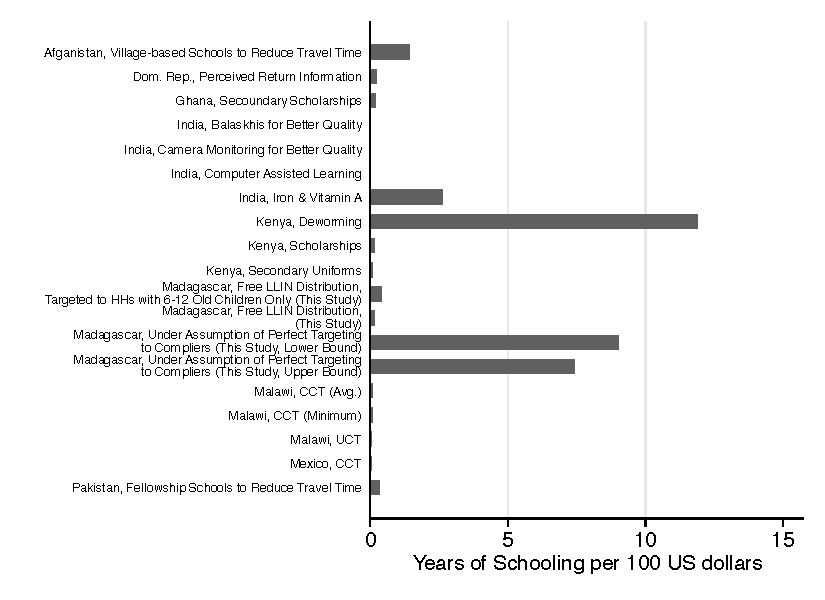
\includegraphics{jpal_yos_new_updated.pdf}
\caption{Comparison of an Additional Year of Schooling for different countries and programs (in hundreds of USD) }
\medskip
\begin{minipage}{0.65\textwidth} % choose width suitably
{\footnotesize Note: The other figures are taken from  \cite{the_abdul_latif_jameel_poverty_action_lab_roll_2017}. Note that these figures take into account a discount rate and are based on 2004 US dollars. For simplicity, our study does not adjust these, but our estimated years of schooling would not change qualitatively, even with these adjustments. \par}
\end{minipage}
\label{jpal_yos}
\end{figure}
%graph hbar  yos,  over(program2,label(labsize( vsmall) ))  leg(off)    ytitle("Years of Schooling per 100 US dollars")  
% graph hbar  yos,  over(program2,relabel( 11 `" "Madagascar, Free LLIN Distribution," "Targeted to HHs with 6-12 Old Children Only (This Study)" "' 12 `" "Madagascar, Free LLIN Distribution," "(This Study)" "'  13 `" "Madagascar, Under Assumption of Perfect Targeting" "to Compliers (This Study, Lower Bound)" "' 14 `" "Madagascar, Under Assumption of Perfect Targeting" "to Compliers (This Study, Upper Bound)" "'  ) label(labsize( vsmall) ))  leg(off)    ytitle("Years of Schooling per 100 US dollars") 

Second, we estimate the total costs and benefits of a free universal distribution. Of our survey respondents, 561 pupils aged 6--12 are enrolled in school. Based on the results in  \autoref{t:absence3rd_questionnaire_child}, which capture the LLIN distribution effects on attendance in the rainy season of the second wave,  the free distribution decreased absences by 1.362 days per person. Assuming zero effects in the dry season again, this implies that, over one year, it increased days of schooling by 561* 1.517  =  764.08  days (i.e., 3.47 years). On the contrary, 1608 nets were actually distributed in the second and third waves, costing USD 2186.88 annually. Therefore, ignoring the delivery cost, 2186.88 / 3.47 = USD 630.22 would be needed for an additional year of schooling. This cost is much higher than the net usage cost of USD 11.12 -- 13.49 required for an additional year of schooling, making the LLIN free distribution program one of the least cost-effective interventions listed in \autoref{jpal_yos}. This high cost can be attributed to the substantial inefficiency in targeting households with children aged 6--12.\footnote{Universal coverage would be less efficient than a perfectly targeted distribution even if we included the targeting cost.
Our household survey cost USD 50,467 during the first wave and there were 216 pupils aged 6—12 years old who were not using nets.
Therefore, we only need 50,467 / 216 + 11.12 (or 13.49) = USD 244.76 (or USD 247.13) for an additional year of schooling by targeting pupils aged 6—12 who are not using nets,
which is USD 407.70 (or USD 410.07) cheaper than universal coverage.} As we can see from \autoref{f:mqnid}, except for those aged 6--20 years old, the respondents' usage rate is as high as 80\%, indicating that the universal free distribution program involves large inclusion errors.\footnote{Admittedly, the comparison assumes there is no social benefit from the free distribution other than the schooling effect for 6--12-year-olds, but it highlights the cost of universal coverage.}



% Second, we estimate the total cost and benefit of free universal distribution. Of our survey respondents, 561 pupils aged 6--12 are enrolled in school. Based on the results in \autoref{t:absence2nd_questionnaire_child_app} and \autoref{t:absence3rd_questionnaire_child}, which capture the LLIN distribution effects on attendance for the second and third waves, respectively, free distribution decreased absence by 1.517 + 1.362  = 2.879 days per person annually, which implies that it increased 561* 2.879  =  1615.12 days (i.e., 7.34 years) of schooling over one year. On the contrary, 1608 nets were actually distributed in the second and third waves, costing 2186.88 US dollars annually. Therefore, ignoring the delivery cost, 2186.88 / 7.34 = 297.88 US dollars would be needed for an additional year of schooling. This cost is much higher than the net usage cost of 7.81 US dollars for an additional year of schooling, making the LLIN free distribution program one of the least cost-effective interventions listed in \autoref{jpal_yos}. This high cost can be attributed to the substantial inefficiency in targeting.\footnote{Universal coverage would be less efficient than perfectly targeted distribution even if we included the targeting cost.
% Our household survey cost 50,467 US dollars during the first wave and there were 216 non-net-using pupils aged 6—12 years old.
% Therefore, we need 50,467 / 216 + 7.81 (or 9.12) = 241.45 (or 242.76) US dollars
% to extend one year of education by targeting non-net-using pupils aged 6--12,
% which is 56.43 (or 55.12) US dollars cheaper than universal coverage.} As we can see from \autoref{f:mqnid}, except for those aged 6--20 years old, respondents' usage rate is as high as 80\%, indicating that the universal free distribution program involves large inclusion errors.\footnote{Admittedly, the comparison assumes there is no social benefit of the free distribution other than the schooling effect for 6--12-year-olds, but it highlights the cost of universal coverage.}
% % % graph hbar yos,over(program2, label(labsize(vsmall ))) ytitle("Years of 

Finally, we suggest a simple but more efficient targeting strategy: excluding households that do not have any children aged 6--12 from the distribution. This strategy is feasible if the government knows citizens' ages or can distribute the mosquito nets at schools. Also, this simple targeting strategy does not require the information about the number of nets possessed by each household.  By excluding households without children aged 6—12 from the distribution campaign, the total number of mosquito nets that the government would have to distribute would decrease from 1608 to 698. This would reduce the distribution cost from USD 2186.88 to USD 949.28, which means that we would need 949.28/ 3.47 = USD 273.57 for an additional year of schooling. This is still much higher than USD 11.12 (or USD 13.49) but this targeted distribution improves efficiency by reducing inclusion errors and becomes more effective than, for example, the fellowship schools program in Pakistan aiming to reduce travel time (\autoref{jpal_yos}).  
% \begin{figure}[h]
% \centering
% \includegraphics[scale=0.3]{ideamap.pdf}
% \caption{Illustration of Empirical Finding}
% \label{ideamap}
% \end{figure}



% Also, because mosquito repellent will increase the quality of sleeping, net using can have good effect on schooling. However, our finding in \autoref{laterdtabsence62} suggests that malaria infection has negative effect on schooling, so even without this kind of sleep quality effect, mosquito net using can have positive affect schooling.

\section{Conclusion}

\label{Feb 12 18:00:13 2013}

By exploiting the natural experiment of the distribution of free LLINs to residents in Madagascar, we
estimated the effect of mosquito net use on schooling. The results from two
data sources, our own panel surveys and school attendance records, show that the LLIN distribution decreased the school absences of pupils aged 6--12 significantly.
Our results suggest that this effect was driven by enhanced mosquito net use and better-controlled malaria infection. Using a mosquito net decreases school absences due to sickness by 16 days per child annually. On the contrary, we found no impact on school enrollment and household-level income, which may affect school enrollment indirectly. Moreover, our finding does not support the existence of any positive externalities arising from LLIN usage. According to our cost--benefit analysis, LLINs costing USD 11.12--13.49 provide an additional year of schooling to pupils aged 6--12. Hence, mosquito nets can be a powerful policy tool for decreasing malaria infections as well as for encouraging human capital investment. In contrast, a universal distribution campaign would cost USD 630.22 for an additional year of schooling, which highlights the significance of its inclusion errors. Such inclusion errors can be reduced when a simple and feasible targeting strategy is adopted: excluding households that do not have any members within the age range targeted by the distribution campaign. This targeting strategy would cut the cost for an additional year of schooling to USD 273.57.

A caveat in this study is that the external validity of these effects and the estimated costs depend on the local climate conditions (e.g., the length of the rainy season). Moreover, the efficiency of the distribution of LLINs depends on the potential mosquito-net usage rate and intra-household allocation to predict who would benefit from such a distribution. These issues are important future research topics.

\bibliographystyle{aer}
\bibliography{malaria,Oriana,Program_evaluation,malariaadd}
% \bibliography{malaria}

\processdelayedfloats
\appendix
\numberwithin{equation}{section}
\numberwithin{figure}{section}
\numberwithin{table}{section}
\section{Appendix}
\renewcommand{\thefigure}{A\arabic{figure}}
\renewcommand{\thepostfigure}{A\arabic{postfigure}}
\setcounter{figure}{0}
\setcounter{postfigure}{0}

This appendix contains a discussion of our estimator, a supplementary analysis, and robustness checks for the main results. \autoref{f:schoolabsence_balance} displays the distribution of absence days in the first wave using the attendance book data. \autoref{drop_2nd3rd_child} analyzes attrition. \autoref{t:ageandclass_2nd} shows a classification of students in the second wave by age and grade. \autoref{t:absence3rd_questionnaire_child_app}, \autoref{t:olsabsence_dailyattend_monthly_withtrend_child_app}, \autoref{mqnidd3rd_child_app}, \autoref{laterdt_child_app}, and \autoref{latemqnabsence62_child_app} present robustness checks for \autoref{t:absence3rd_questionnaire_child}, \autoref{t:olsabsence_dailyattend_monthly_withtrend_child}, \autoref{mqnidd3rd_child}, \autoref{laterdt_child}, and \autoref{latemqnabsence62_child}, respectively.  \autoref{floornetusing} analyzes why children aged 6--12 did not use mosquito nets, based on the first-wave data. \autoref{distributionknow} examines the announcement effect by excluding households that knew about the free distribution campaign one wave before it was conducted. \autoref{ivandols} compares the OLS and IV regression results. 
% The survey questionnaire we used in the third wave follows after these figures and tables.

\subsection{Seasonality and Learning Effects}
\subsubsection{Setting}
We reintroduce a true model to focus on what the Difference-in-Differences or IV estimators in \autoref{latemqnabsence62_child} capture. Suppose the following model is the true model describing the relationship between the outcome (attendance, $Y$) and treatment variable (net use, $N$).
\begin{gather*}
E[Y_{ijt}] = \alpha_{it} N_{ijt} + \eta_{t} + \mu_{j} 
\end{gather*}
where $i$ represents an individual, $j$ the village, and $t$ is time. $\eta_{t} $ and $\mu_{j}$ are fixed effects.
The DID reduced-form effect using the 2nd and 3rd waves is
\begin{gather}
% E[Y_{ij3}|G] - E[Y_{ij2}|G] =  E[\alpha_{i3} N_{ij3} - \alpha_{i2} N_{ij2}|G] + \eta_{3} - \eta_{2} \\
E[Y_{ij3}|G=0] - E[Y_{ij2}|G=0]  - \left(E[Y_{ij3}|G=1] - E[Y_{ij2}|G=1] \right) \notag \\
=E[Y_{ij2}|G=1] - E[Y_{ij2}|G=0]  + \left(E[Y_{ij3}|G=0] - E[Y_{ij3}|G=1] \right)\notag \\
 =  \left( E[\alpha_{i2} N_{ij2}|G=1]   - E[\alpha_{i2}N_{ij2}|G=0]\right) +  \left(  E[\alpha_{i3}N_{ij3}|G=0] - E[\alpha_{i3} N_{ij3}|G=1]  \right),
\end{gather}
where $G=1$ ($G=0$) is south (north), which received nets in the second (third) wave. 

Suppose the following model is the true model describing the relationship between the treatment variable and the distribution ($D$).
\begin{gather*}
E[N_{ijt}] = \beta_{it} D_{jt} + \gamma_{it} L.D_{jt} +  \xi_{t} + \psi_{j}, 
\end{gather*}
where $\xi_{t} $ and $\psi_{j}$ are fixed effects and $L.D$ is a lag of $D$.  $\gamma_{it}$ is a learning effect: some people may stop using nets half a year after the distribution, after realizing their low effectiveness. The DID estimator for the first stage is
\begin{gather*}
E[N_{ij3}|G=0] - E[N_{ij2}|G=0]  - \left(E[N_{ij3}|G=1] - E[N_{ij2}|G=1] \right) \\
=\left( E[\beta_{i2} D_{j2}|G=1]   - E[\beta_{i2}D_{j2}|G=0]\right) +  \left(  E[\beta_{i3}D_{j3}|G=0] - E[\beta_{i3} D_{j3}|G=1]  \right) \\
\quad +  \left(  E[\gamma_{3i}L.D_{j3}|G=0] - E[\gamma_{3i} L.D_{j3}|G=1]  \right) .
\end{gather*}
The second term will be zero because the distribution effect $\beta_{i3}$ is assumed to be the same in the two regions. The third term will be equal to $- E[\gamma_{3i} L.D_{j3}|G=1]$ because the learning effect will be zero in the third wave for $G=0$, as households in this region have only recently received nets. Therefore, the DID estimator for the first stage will correspond to $\left( E[\beta_{i2} D_{j2}|G=1]   - E[\beta_{i2}D_{j2}|G=0]\right)  - E[\gamma_{3i} L.D_{j3}|G=1] $.

\subsubsection{Zero-Learning Effect Case}
When $\gamma_{it} = 0$ for all individuals, $ - E[\gamma_{3i} L.D_{j3}|G=1] = 0$. Further,  
 $ \left(  E[\alpha_{i3}N_{ij3}|G=0] - E[\alpha_{i3} N_{ij3}|G=1] \right) $ in equation (1) will be zero because both regions would show the same level of attendance in the third phase after controlling for fixed effects. 


The Wald estimator (equal to 2SLS after taking the first difference) using the DID estimators above as the denominator and numerator becomes 
\begin{gather*}
\frac{ E[\alpha_{i2} N_{ij2}|G=1]   - E[\alpha_{i2}N_{ij2}|G=0]}{ E[\beta_{i2} D_{j2}|G=1]   -E[\beta_{i2}D_{j2}|G=0]} .
\end{gather*}
and this will be the LATE for the effect in the second wave for people who will start using a net because of the distribution in the second wave. This is the standard result in the literature. A corollary of this result is that we only capture the effect in the second wave (rainy season), not in the third wave. Therefore, when we calculate the cost effectiveness per year, we have to assume a value for the effect in the dry season; in the main text, we used 0 to be conservative.


\subsubsection{Non-zero Learning Effect Case}
When $\gamma_{it}$ is not zero, the Wald estimator will be 
\begin{gather}
\frac{\left( E[\alpha_{i2} N_{ij2}|G=1]   - E[\alpha_{i2}N_{ij2}|G=0]\right) +  \left(  E[\alpha_{i3}N_{ij3}|G=0] - E[\alpha_{i3} N_{ij3}|G=1]  \right)}{\left( E[\beta_{i2} D_{j2}|G=1]   - E[\beta_{i2}D_{j2}|G=0]\right)  - E[\gamma_{3i} L.D_{j3}|G=1]
}.
\end{gather}
Because some people stopped using nets in $G=1$ ($\gamma_{it}<0$ on average) in the third wave, the second term in the denominator will be positive and the denominator will be larger. The numerator will be also larger because  $N_{ij3}$ will be smaller for $G=1$ on average. Therefore, we cannot predict whether the DID estimator might show a larger or smaller effect compared to the zero-learning effect case. 

However, consider a very plausible case: when people stop using nets ($\gamma_{3i} < 0 $) only if their effect ($\alpha_{i3}$) is zero and other people keep using nets, $\gamma_{3i} = 0 $ because $\alpha_{i3}>0$. We call this the case of disappointment. Then,

\begin{gather*}
E[\alpha_{i3}N_{ij3}|G=0] - E[\alpha_{i3} N_{ij3}|G=1]  \\
 =  Pr(\gamma_{i3} =0 )\left[E[\alpha_{i3}N_{ij3}| \gamma_{3i} = 0, G=0] - E[\alpha_{i3} N_{ij3}|\gamma_{3i} = 0, G=1] \right] \\
 + Pr(\gamma_{i3} <0 )\left[E[\alpha_{i3}N_{ij3}| \gamma_{3i} < 0, G=0] - E[\alpha_{i3} N_{ij3}|\gamma_{3i} < 0, G=1] \right] \\
  =  Pr(\gamma_{i3} =0 )\left[E[\alpha_{i3}N_{ij3}| \gamma_{3i} = 0, G=0] - E[\alpha_{i3} N_{ij3}|\gamma_{3i} = 0, G=1] \right] \\
 + Pr(\gamma_{i3} <0 )\left[E[\alpha_{i3}N_{ij3}| \alpha_{i3} = 0, G=0] - E[\alpha_{i3} N_{ij3}|\alpha_{i3} = 0, G=1] \right] 
 \\ = 0 + 0 
\end{gather*}
assuming $F(\gamma_{it}|G) = F(\gamma_{it})$ and $F(\alpha_{i3}N_{ij3}|\gamma_{3i}, G) = F(\alpha_{i3}N_{ij3}|\gamma_{3i}) $. The first term is zero because the terms in the brackets will cancel each other out, and the second term is zero because $\alpha_{i3}=0$.
Therefore, in this case, only the denominator will increase and the Wald estimator will show a smaller effect than that in the zero-learning effect case.


When using the data in the second wave to conduct a cross-sectional 2SLS, we will estimate the LATE without a learning effect. In that case,  the difference between the cross-sectional 2SLS and DID-IV estimates (columns (1)--(3) and (4)--(6) in Panel A of  \autoref{latemqnabsence62_child}) would be explained by the population parameter to be estimated and the bias would stem from the fixed effects. 
If the bias is not the issue (the cross-sectional 2SLS identifies the LATE), then we will obtain a point estimate similar to that with DID-IV by restricting the sample to those using nets in the third period ($N_{i3}=1$) because these people would exhibit a small learning effect.

In Panel B of  \autoref{latemqnabsence62_child}, we use malaria infection as a treatment variable and do not observe a difference between columns (1)--(3) and (4)--(6). This is because the presence of learning effects will not change the reduced-form impacts on school absences, the numerator of the Wald estimator. The denominator of the Wald estimator in Panel B, the reduced-form impact on malaria infection, will not change by the learning effect when we consider the case of disappointment in malaria infection. Therefore, both the cross-sectional 2SLS and DID-IV will estimate the same population parameter.



\begin{figure}[h]
\centering
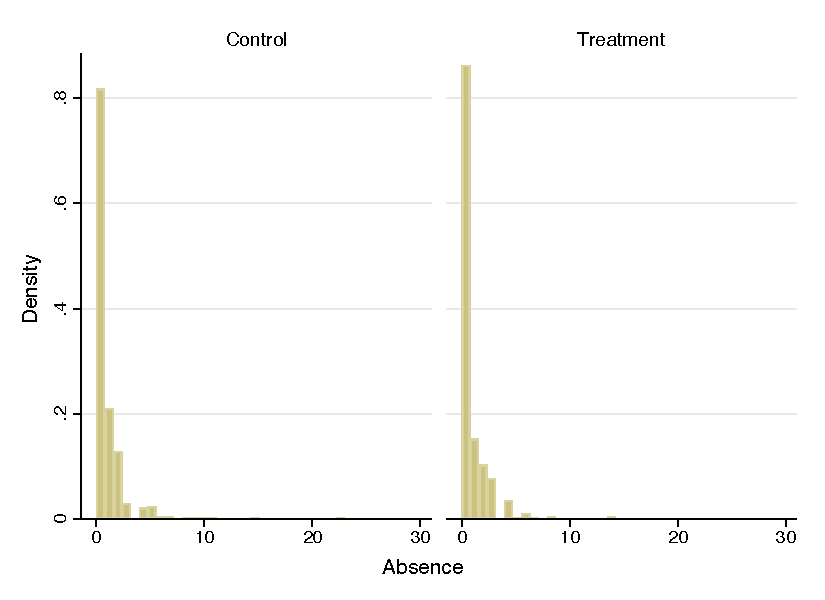
\includegraphics[scale=0.8]{schoolabsence_balance.pdf}
\caption{Distribution of Absence Days in the First Wave (Based on Attendance Book Data)}
\label{f:schoolabsence_balance}
\floatfoot{\textit{Notes:} This graph shows the distribution of absence days recorded in the attendance book in the first wave (June 2009 -- December 2009).}

\end{figure}



\begin{table}[h]
\caption{Attrition}
\label{drop_2nd3rd_child}\centering
\begin{adjustbox}{max width=\textwidth}
\begin{threeparttable}
\begin{tabular}{l*{5}{c}}
\hline\hline

                    &\multicolumn{5}{c}{Dropped After the First Wave}\\ \cmidrule(lr){2-6} 
                                     Variables in the First Wave &\multicolumn{1}{c}{(1)}&\multicolumn{1}{c}{(2)}&\multicolumn{1}{c}{(3)}&\multicolumn{1}{c}{(4)}&\multicolumn{1}{c}{(5)}\\
\hline
RDT +               &      0.0381         &                     &                     &                     &      0.0306         \\
                    &    (0.0230)         &                     &                     &                     &    (0.0215)         \\

Sleep under a Net      &                     &   -0.000607         &                     &                     &     0.00557         \\
                    &                     &    (0.0102)         &                     &                     &   (0.00874)         \\

Absence Last Month  &                     &                     &     0.00377         &                     &     0.00340         \\
                    &                     &                     &   (0.00297)         &                     &   (0.00299)         \\

Household size             &                     &                     &                     &    -0.00654\sym{+}  &    -0.00459         \\
                    &                     &                     &                     &   (0.00316)         &   (0.00347)         \\

Constant            &      0.0181\sym{**} &      0.0231\sym{*}  &      0.0126         &      0.0564\sym{*}  &      0.0292         \\
                    &   (0.00555)         &    (0.0107)         &   (0.00879)         &    (0.0213)         &    (0.0237)         \\
\hline
N                   &         696         &         704         &         557         &         704         &         550         \\
F\_test              &                     &                     &                     &                     &       1.778         \\
\hline\hline
\end{tabular}
\begin{tablenotes}
\item Cluster-robust standard errors (18 village-level with a finite sample adjustment) are in parentheses. We only use data from the first wave. 
\end{tablenotes}
\end{threeparttable}
\end{adjustbox}
\end{table}




\begin{table}[h]
\caption{Classification by Age and Grade}
\label{t:ageandclass_2nd}\centering
\begin{adjustbox}{max width=\textwidth}
\begin{threeparttable}
\begin{tabular}{l*{5}{c}}
\hline\hline
            &\multicolumn{5}{c}{Grade}                                            \\
       &          1&          2&          3&          4&          5\\
    Age         &  \quad     &    \quad   &    \quad   &    \quad   &   \quad    \\
\hline
1           &           1&           0&           0&           0&           0\\
4           &           1&           0&           1&           0&           0\\
5           &          13&           0&           0&           0&           0\\
6           &          38&           2&           1&           0&           1\\
7           &          70&          23&           1&           0&           1\\
8           &          44&          39&           5&           0&           0\\
9           &          25&          35&          30&           0&           0\\
10          &           8&          39&          42&          14&           2\\
11          &           5&          12&          33&          19&           1\\
12          &           5&          12&          29&          16&          12\\
13          &           3&           5&          12&          23&           7\\
14          &           0&           3&           9&          13&           9\\
15          &           0&           0&           3&           2&           6\\
16          &           0&           1&           3&           1&           1\\
17          &           0&           0&           1&           1&           0\\
18          &           0&           0&           0&           1&           0\\
\hline\hline
\end{tabular}
\begin{tablenotes}
\item We used the pupils from the second wave.
\end{tablenotes}
\end{threeparttable}
\end{adjustbox}

\end{table}

\begin{table}[h]
\caption{Robustness Check: Effect of Net Distribution on Schooling (Based on the Survey Data)}
\label{t:absence3rd_questionnaire_child_app}\centering
\begin{adjustbox}{max width=\textwidth}
\begin{threeparttable}
\begin{tabular}{l*{7}{c}}
\hline\hline
          &\multicolumn{3}{c}{Sick Absence (6 Months)}&\multicolumn{3}{c}{Absence (6 Months)}\\   \cmidrule(lr){2-4} \cmidrule(lr){5-7}
            \textit{Panel A: Absence}                  &\multicolumn{1}{c}{(1)}&\multicolumn{1}{c}{(2)}&\multicolumn{1}{c}{(3)}&\multicolumn{1}{c}{(4)}&\multicolumn{1}{c}{(5)}&\multicolumn{1}{c}{(6)}\\

\hline
Distributed         &        -1.362\sym{*}  &      -1.242\sym{*}  &      -1.216\sym{*} & -3.095\sym{*}  &      -1.222         &      -0.914      \\
 &       (0.602)         &       (0.462)         &       (0.487)         &       (1.432)         &       (0.888)         &       (0.774)         \\

Individual Fixed Effects and Wave Fixed Effects &         Yes         &         Yes         &         Yes         &         Yes         &         Yes         &         Yes         \\

Pre-village-level Absence * Wave Fixed Effects&          No         &         Yes         &         Yes         &          No         &         Yes         &         Yes         \\

Pre-high Malaria Risk Village * Wave Fixed Effects&          No         &          No         &         Yes         &          No         &          No         &         Yes         \\

Pre-village-level Net Use * Wave Fixed Effects&          No         &          Yes         &         Yes        &     No         &          Yes         &         Yes       \\

Altitude * Wave Fixed Effects&          No         &          No         &         Yes        &     No         &          No         &         Yes        \\
\hline
p-value&               0.038         &       0.016         &       0.024 &     0.046         &       0.188         &       0.255              \\
Wild Bootstrap p-value &          0.045         &       0.065         &       0.076         &       0.072         &       0.301         &       0.318       \\
Number of Observations        &        1122         &        1122         &        1122         &        1122         &        1122         &        1122         \\
\\
                      &\multicolumn{3}{c}{Enrollment} &&& \\  \cmidrule(lr){2-4} 
                    
        \textit{Panel B: Enrollment}                   &\multicolumn{1}{c}{(1)}&\multicolumn{1}{c}{(2)}&\multicolumn{1}{c}{(3)} &&& \\
\hline
Distributed         &     -0.0384         &     -0.0305         &     -0.0288         \\
                    &    (0.0222)         &    (0.0244)         &    (0.0262)         \\

Individual Fixed Effects and Wave Fixed Effects &         Yes         &         Yes         &         Yes        &&& \\

Pre-village-level Enrollment * Wave Fixed Effects&          No         &         Yes         &         Yes        &&& \\

Pre-high Malaria Risk Village * Wave Fixed Effects&          No         &          Yes         &         Yes        &&& \\

Pre-village-level Net Use * Wave Fixed Effects&          No         &          Yes         &         Yes        &&& \\

Altitude * Wave Fixed Effects&          No         &          No         &         Yes        &&& \\
\hline
p-value     &       0.102         &       0.228         &       0.287     &&&\\
Wild Bootstrap p-value &       0.064         &       0.270         &       0.431  &&&\\       
Number of Observations        &        2147         &        2147         &        2147        &&& \\
\hline\hline
\end{tabular}
\begin{tablenotes}
\item Cluster-robust standard errors (18 village-level with a finite sample adjustment) are in parentheses. \sym{+} \(p<.10\), \sym{*} \(p<.05\), \sym{**} \(p<.01\), and \sym{***} \(p<.001\). In Panel A, we only use the second and third waves. In Panel B, we use all the waves.
\end{tablenotes}
\end{threeparttable}
\end{adjustbox}
\end{table}




\begin{table}[h]
\caption{Effect of Net Distribution on the Absence Rate (Based on the School Attendance
Book Data)}
\label{t:olsabsence_dailyattend_monthly_withtrend_child_app}\centering
\begin{adjustbox}{max width=\textwidth}
\begin{threeparttable}
\begin{tabular}{l*{5}{c}}
\hline\hline
&\multicolumn{5}{c}{Monthly Absence Rate}\\ \cmidrule(lr){2-6}
                    &\multicolumn{1}{c}{(1)}&\multicolumn{1}{c}{(2)}&\multicolumn{1}{c}{(3)}&\multicolumn{1}{c}{(4)}&\multicolumn{1}{c}{(5)}\\\hline
Distributed          &     -0.0131\sym{*}  &     -0.0127\sym{*}  &     -0.0125\sym{*}  &     -0.0102\sym{+}  &     -0.0167\sym{+}  \\
            &    (0.00557)         &     (0.00597)         &     (0.00588)         &     (0.00570)         &     (0.00978)         \\

School Fixed Effects           &         Yes         &         Yes         &         Yes         &         Yes         &         Yes         \\

Wave Fixed Effects            &         Yes         &         Yes         &         Yes         &         Yes         &         Yes         \\

Season Fixed Effects            &          No         &          No         &         Yes         &         Yes         &          Yes         \\

Linear Trend * School Fixed Effects &          No         &          No         &          No         &         Yes         &          No         \\

Season * School Fixed Effects   &          No         &          No         &          No         &          No         &         Yes         \\
\hline
p-value          &       0.026         &       0.042         &       0.043         &       0.085         &       0.097         \\
Wild Bootstrap p-value  &       0.055         &       0.059         &       0.064         &       0.152         &       0.175         \\
Number of Observations        &       13928         &       19104         &       19104         &       19104         &       19104         \\
\hline\hline
\end{tabular}
\begin{tablenotes}
\item The 31 grade * school-level cluster robust standard errors are in parentheses. The \textit{p-value} and \textit{Wild Bootstrap p-value} are used to test whether the treatment coefficient is zero, using the standard error in the table and the cluster-robust wild bootstrap, respectively. \sym{+} \(p<.10\), \sym{*} \(p<.05\), \sym{**} \(p<.01\), and \sym{***} \(p<.001\). Column (1) uses data only after June 2009 as in the survey data results, whereas the other columns include December 2008--July 2009. \textit{Season Fixed Effects} capture monthly seasonal effects, taking the value of one for January, for example.
\end{tablenotes}
\end{threeparttable}
\end{adjustbox}
\end{table}



\begin{table}[h]
\caption{Robustness Check: Effect of Net Distribution on the Usage Rate}
\label{mqnidd3rd_child_app}
\centering
\begin{adjustbox}{max width=\textwidth}
\begin{threeparttable}
\begin{tabular}{l*{4}{c}}
\hline\hline
	&\multicolumn{4}{c}{Sleep under a Net}\\  \cmidrule(lr){2-5}
	&\multicolumn{2}{c}{All Ages}&\multicolumn{2}{c}{6--12 Years Old}\\ \cmidrule(lr){2-3}  \cmidrule(lr){4-5}
                    &\multicolumn{1}{c}{(1)}&\multicolumn{1}{c}{(2)}&\multicolumn{1}{c}{(3)}&\multicolumn{1}{c}{(4)}\\
    \multicolumn{4}{l}{\textit{Panel A: All Households}}  \\ \hline
Distributed         &       0.129\sym{***}&       0.119\sym{***}&       0.154\sym{**} &       0.190\sym{***}\\
                    &    (0.0247)         &    (0.0278)         &    (0.0413)         &    (0.0373)         \\
   \multicolumn{4}{l}{\textit{Panel B: All Households with More than 0.5 Nets per Member in the First Wave}} \\ \hline


   Distributed         &      0.0437         &     0.00549         &     -0.0561         &     -0.0490         \\
                    &      (0.0368)         &      (0.0366)         &      (0.0464)         &      (0.0620)         \\
Individual Fixed Effects and Wave Fixed Effects &         Yes         &         Yes         &         Yes         &         Yes         \\

Pre-village-level Absence * Wave Fixed Effects&          No         &         Yes         &          No         &         Yes     \\

Pre-high Malaria Risk Village * Wave Fixed Effects&          No         &          Yes         &     No         &         Yes     \\

Pre-village-level Net Use * Wave Fixed Effects&          No         &          Yes         &        No         &         Yes    \\

Altitude * Wave Fixed Effects&          No         &          Yes         &        No         &         Yes     \\
\hline
 p-value in Panel A                   &       0.000         &       0.001         &       0.002         &       0.000         \\
Wild Bootstrap p-value in Panel A&       0.000         &       0.012         &       0.017         &       0.020         \\
Number of Observations in Panel A       &       11232         &       11232         &        2148         &        2148         \\
Number of Observations in Panel B        &        1671         &        1671         &         181         &         181         \\

\hline\hline
\end{tabular}
\begin{tablenotes}
\item Cluster-robust standard errors (18 village-level with a finite sample adjustment) are in parentheses. In panel A, we use all households, while we only use households that had more than 0.5 nets per member in the first wave per member. Columns (1) and (2) use the sample of children aged 6--12 and the other samples whereas columns (3) and (4) only use the sample of children aged 6--12. The \textit{p-value} and \textit{Wild Bootstrap p-value} are used to test whether the treatment coefficient is zero, using the standard error in the table and the cluster-robust wild bootstrap, respectively. Data from all the waves are used.\sym{+} \(p<.10\), \sym{*} \(p<.05\), \sym{**} \(p<.01\), and \sym{***} \(p<.001\). \end{tablenotes}
\end{threeparttable}
\end{adjustbox}
\end{table}


\begin{table}[h]
\caption{Why Do Children Not Sleep under Mosquito Nets?}
\label{floornetusing}
\centering
\begin{adjustbox}{max width=\textwidth}
\begin{threeparttable}
\begin{tabular}{l*{5}{c}}
\hline\hline
	&\multicolumn{5}{c}{Sleep under a Net}\\  \cmidrule(lr){2-6}

                    &\multicolumn{1}{c}{(1)}&\multicolumn{1}{c}{(2)}&\multicolumn{1}{c}{(3)}&\multicolumn{1}{c}{(4)}&\multicolumn{1}{c}{(5)}\\

\hline
6--12 years old      &      -0.133\sym{***}&     -0.0817\sym{**} &      -0.127\sym{***}&     -0.0770\sym{*}  &     -0.0716\sym{*}  \\
                    &    (0.0263)         &    (0.0280)         &    (0.0280)         &    (0.0295)         &    (0.0281)         \\

Sleep on the Floor               &                     &      -0.195\sym{***}&                     &      -0.193\sym{***}&      -0.206\sym{***}\\
                    &                     &    (0.0253)         &                     &    (0.0247)         &    (0.0287)         \\

No. of Household Members Children Sleep With          &                     &                     &      0.0440\sym{*}  &      0.0415\sym{*}  &       0.108\sym{***}\\
                    &                     &                     &    (0.0168)         &    (0.0164)         &    (0.0193)         \\
                    
Household FEs         &   No                   &   No                   &   No      &   No     &  Yes   \\

\hline
Number of Observations        &        3249         &        3249         &        3249         &        3249         &        3249         \\
\hline\hline
\end{tabular}
\begin{tablenotes}
\item Cluster-robust standard errors (18 village-level with a finite sample adjustment) are in parentheses. \sym{+} \(p<.10\), \sym{*} \(p<.05\), \sym{**} \(p<.01\), and \sym{***} \(p<.001\). We use the first-wave data.
\end{tablenotes}
\end{threeparttable}
\end{adjustbox}
\end{table}





\begin{table}[h]
\caption{Robustness Check: Effect of Mosquito Net Use on Malaria Infection}
\label{laterdt_child_app}\centering
\begin{adjustbox}{max width=\textwidth}
\begin{threeparttable}
\begin{tabular}{l*{6}{c}}
\hline\hline
&\multicolumn{6}{c}{RDT +}\\     \cmidrule(lr){2-7}
                                        &\multicolumn{3}{c}{2SLS (Second Wave)}&\multicolumn{3}{c}{FE-IV (All Waves)}\\  \cmidrule(lr){2-4}  \cmidrule(lr){5-7}

                    &\multicolumn{1}{c}{(1)}&\multicolumn{1}{c}{(2)}&\multicolumn{1}{c}{(3)}&\multicolumn{1}{c}{(4)}&\multicolumn{1}{c}{(5)}&\multicolumn{1}{c}{(6)}\\

\hline
Sleep under a Net      &      -1.094\sym{*}  &      -0.713\sym{**} &      -0.415\sym{*}  &      -0.620\sym{*}  &      -0.528\sym{*}  &      -0.533\sym{*}  \\
                    &     (0.462)         &     (0.187)         &     (0.151)         &     (0.254)         &     (0.225)         &     (0.231)         \\

Individual Fixed Effects and Wave Fixed Effects &          No         &          No         &          No         &         Yes         &         Yes         &         Yes         \\

Pre-high Malaria Risk Village * Wave Fixed Effects&          No         &         Yes         &         Yes         &          No         &         Yes         &         Yes         \\

Pre-village-level Infection Rate  * Wave Fixed Effects&          No         &          No         &          Yes         &          No         &          No         &         Yes         \\

Pre-village-level Absence * Wave Fixed Effects&          No         &         Yes         &         Yes        & No         &         Yes         &         Yes      \\

Pre-village-level Net Use * Wave Fixed Effects&         No         &         Yes         &         Yes        & No         &         Yes         &         Yes    \\

Altitude * Wave Fixed Effects&         No         &         Yes         &         Yes        & No         &         Yes         &         Yes   \\
\hline
         p-value           &       0.030         &       0.001         &       0.014         &       0.026         &       0.032         &       0.034         \\
Wild Bootstrap p-value &       0.008         &       0.006         &       0.047         &       0.014         &       0.055         &       0.082         \\

Number of Observations        &         696         &         696         &         696         &        2043         &        2043         &        2043         \\
\hline\hline
\end{tabular}
\begin{tablenotes}
\item Cluster-robust standard errors (18 village-level with a finite sample adjustment) are in parentheses. \sym{+} \(p<.10\), \sym{*} \(p<.05\), \sym{**} \(p<.01\), and \sym{***} \(p<.001\). In columns (1)--(3), we only use the second wave. In columns (4)--(6), we only use the second and third waves. 

\end{tablenotes}
\end{threeparttable}
\end{adjustbox}
\end{table}



\begin{table}[h]
\caption{Robustness Check: Effect of Mosquito Net Use or Malaria Infection on Schooling}
\label{latemqnabsence62_child_app}\centering
\begin{adjustbox}{max width=\textwidth}
\begin{threeparttable}
\begin{tabular}{l*{6}{c}}
\hline\hline
                                                                \\
                                                                 &\multicolumn{6}{c}{Sick Absence (6 months)}\\  \cmidrule(lr){2-7}

                                       &\multicolumn{3}{c}{2SLS (Second Wave)}&\multicolumn{3}{c}{FE-IV (second \& third Waves)}\\  \cmidrule(lr){2-4}  \cmidrule(lr){5-7}
                    &\multicolumn{1}{c}{(1)}&\multicolumn{1}{c}{(2)}&\multicolumn{1}{c}{(3)}&\multicolumn{1}{c}{(4)}&\multicolumn{1}{c}{(5)}&\multicolumn{1}{c}{(6)}\\
                       \multicolumn{6}{l}{\textit{Panel A: Effect of Mosquito Net Use}}\\  \hline

Sleep under a Net      &      -13.45\sym{+}  &      -10.33\sym{**} &      -10.47\sym{**} &      -5.701\sym{+}  &      -5.038\sym{**} &      -5.130\sym{*}  \\
                    &     (7.051)         &     (3.117)         &     (3.396)         &     (2.940)         &     (1.592)         &     (2.148)         \\

                       \multicolumn{6}{l}{\textit{Panel B: Effect of Malaria Infection}}\\  \hline

RDT +               &       11.26\sym{*}  &       9.840\sym{*}  &       14.68\sym{***}&       13.92\sym{+}  &       16.95\sym{+}  &       18.56\sym{+}  \\
                    &     (4.507)         &     (4.356)         &     (3.483)         &     (7.313)         &     (8.381)         &     (10.41)         \\

Individual Fixed Effects and Wave Fixed Effects &          No         &          No         &          No         &         Yes         &         Yes         &         Yes         \\

Pre-village-level Absence * Wave Fixed Effects&          No         &         Yes         &         Yes         &          No         &         Yes         &         Yes         \\

Pre-high Malaria Risk Village * Wave Fixed Effects &          No         &          No         &         Yes         &          No         &          No         &         Yes         \\
Pre-village-level Net Use * Wave Fixed Effects&         No         &         Yes         &         Yes        & No         &         Yes         &         Yes    \\

Altitude * Wave Fixed Effects&         No         &         Yes         &         Yes        & No         &         Yes         &         Yes   \\
\hline
   p-value  in Panel A&       0.074         &       0.004         &       0.007         &       0.070         &       0.006         &       0.030  \\
  Wild Bootstrap p-value  in Panel A&       0.051         &       0.065         &       0.094         &       0.066         &       0.031         &       0.082  \\    
Number of Observations in Panel A       &         573         &         573         &      573         &        1122  &    1122         &        1122         \\
            p-value in Panel B         &       0.024         &       0.038         &       0.001         &       0.075         &       0.060         &       0.094         \\
Wild Bootstrap p-value in Panel B &       0.013         &       0.145         &       0.026         &       0.027         &       0.053         &       0.081         \\

Number of Observations in Panel B       &          563         &         563         &         563         &        1002         &        1002         &        1002            \\
\hline\hline
\end{tabular}
\begin{tablenotes}
\item Cluster-robust standard errors (18 village-level with a finite sample adjustment) are in parentheses. We use distribution as an instrument. \sym{+} \(p<.10\), \sym{*} \(p<.05\), \sym{**} \(p<.01\), and \sym{***} \(p<.001\). In columns (1)--(3), we only use the second wave. In columns (4)--(6), we only use the second and third waves. 
\end{tablenotes}
\end{threeparttable}
\end{adjustbox}
\end{table}

\begin{table}[h]
\caption{Result Excluding Households that Knew About the Free Distribution One Wave Before it was Conducted}
\label{distributionknow}
\centering
\centering
\begin{adjustbox}{max width=\textwidth}
\begin{threeparttable}
\begin{tabular}{l*{4}{c}}
\hline\hline                                        &\multicolumn{2}{c}{FE}&\multicolumn{2}{c}{FE-IV}\\ \cmidrule(lr){2-3}\cmidrule(lr){4-5}

                    &\multicolumn{1}{c}{Sick Absence (6 months)}&\multicolumn{1}{c}{Sleep under a Net}&\multicolumn{1}{c}{RDT +}&\multicolumn{1}{c}{Sick Absence (6 months)}\\
                                                            &\multicolumn{1}{c}{(1)}&\multicolumn{1}{c}{(2)}&\multicolumn{1}{c}{(3)}&\multicolumn{1}{c}{(4)}\\
\hline
Distributed         &      -1.214\sym{+}  &       0.161\sym{**} &                     &                     \\
                    &     (0.609)         &    (0.0464)         &                     &                     \\
Sleep under a Net      &                     &                     &      -0.553\sym{*}  &      -4.912\sym{+}  \\
                    &                     &                     &     (0.235)         &     (2.749)         \\
\hline
Wave Fixed Effects and Individual Fixed Effects & Yes & Yes & Yes& Yes \\
 p-value   &       0.064         &       0.003      &       0.031         &       0.093         \\
  Wild Bootstrap p-value &       0.073         &       0.015         &       0.011         &       0.093         \\
Number of Observations        &        1068         &        2016         &        1926         &        1068         \\
\hline\hline
\end{tabular}
\begin{tablenotes}
\item Cluster-robust standard errors (18 village-level with a finite sample adjustment) are in parentheses. \sym{+} \(p<.10\), \sym{*} \(p<.05\), \sym{**} \(p<.01\), and \sym{***} \(p<.001\). Columns (1) and (4) use the second and third waves and columns (2) and (3) use all waves.

\end{tablenotes}

\end{threeparttable}
\end{adjustbox}
\end{table}

\begin{table}[h]
\caption{Comparison between IV and OLS}
\label{ivandols}
\centering
\begin{adjustbox}{max width=\textwidth}
\begin{threeparttable}
\begin{tabular}{l*{4}{c}}
\hline\hline
                                        &\multicolumn{2}{c}{RDT +}&\multicolumn{2}{c}{Sick Absence (6 Months)}                   \\ \cmidrule(lr){2-3} \cmidrule(lr){4-5}
                                                            &\multicolumn{1}{c}{OLS}&\multicolumn{1}{c}{IV}&\multicolumn{1}{c}{OLS}&\multicolumn{1}{c}{IV}\\
                    &\multicolumn{1}{c}{(1)}&\multicolumn{1}{c}{(2)}&\multicolumn{1}{c}{(3)}&\multicolumn{1}{c}{(4)}\\

\hline
Sleep under a Net      &      -0.150\sym{***}&      -0.442\sym{**} &       0.980\sym{*}  &      -13.45\sym{+}  \\
                    &    (0.0312)         &     (0.132)         &     (0.459)         &     (7.059)         \\

Village-level Infection in the First Wave&       Yes&       Yes&  No                    &  No                    \\

Village-level Sick Absence in the First Wave&   No                   &   No                   &       Yes        &      Yes      \\

\hline \
Number of Observations        &         696         &         696         &         573         &         573         \\ \hline\hline
\end{tabular}
\begin{tablenotes}
\item Cluster-robust standard errors (18 village-level with a finite sample adjustment) are in parentheses. \sym{+} \(p<.10\), \sym{*} \(p<.05\), \sym{**} \(p<.01\), and \sym{***} \(p<.001\) We only use the second wave of data.
\end{tablenotes}
\end{threeparttable}
\end{adjustbox}

\end{table}

% \begin{table}[h]
% \caption{Robustness Check: The Effect of the Distribution on Schooling Using Only the Second Wave (From the Survey)}
% \label{t:absence2nd_questionnaire_child_app}\centering
% \begin{adjustbox}{max width=\textwidth}
% \begin{threeparttable}
% \begin{tabular}{l*{7}{c}}
% \hline\hline
%           &\multicolumn{3}{c}{Sick Absence (6 Months)}&\multicolumn{3}{c}{Absence (6 Months)}\\   \cmidrule(lr){2-4} \cmidrule(lr){5-7}
%    &\multicolumn{1}{c}{(1)}&\multicolumn{1}{c}{(2)}&\multicolumn{1}{c}{(3)}&\multicolumn{1}{c}{(4)}&\multicolumn{1}{c}{(5)}&\multicolumn{1}{c}{(6)}\\
% \hline
% Distributed          &      -1.517\sym{*}  &      -1.478\sym{**} &      -1.296\sym{*}  &      -3.372\sym{*}  &      -1.488         &      -1.253         \\
%             &       (0.533)         &       (0.422)         &       (0.483)         &       (1.463)         &       (0.883)         &       (0.817)         \\

% Individual Fixed Effects and Wave Fixed Effects &         Yes         &         Yes         &         Yes         &         Yes         &         Yes         &         Yes         \\

% Pre-village-level Absence * Wave Fixed Effects&          No         &         Yes         &         Yes         &          No         &         Yes         &         Yes         \\

% Pre-high Malaria Risk Village * Wave Fixed Effects&          No         &          No         &         Yes         &          No         &          No         &         Yes         \\

% Pre-village-level Net Use * Wave Fixed Effects&          No         &          Yes         &         Yes        &     No         &          Yes         &         Yes       \\

% Altitude * Wave Fixed Effects&          No         &          No         &         Yes        &     No         &          No         &         Yes        \\
% \hline
% p-value               &       0.012         &       0.003         &       0.016         &       0.035         &       0.112         &       0.145               \\
% Wild Bootstrap p-value             &       0.001         &       0.155         &       0.130         &       0.002         &       0.499         &       0.472         \\
% Observations        &         573         &         573         &         573         &         573         &         573         &         573           \\
% \hline\hline
% \end{tabular}
% \begin{tablenotes}
% \item Cluster-robust standard errors (18 village level with finite sample adjustment) are in parentheses. \sym{+} \(p<.10\), \sym{*} \(p<.05\), \sym{**} \(p<.01\), \sym{***} \(p<.001\). We only use the second and third waves. 
% \end{tablenotes}
% \end{threeparttable}
% \end{adjustbox}
% \end{table}

\end{document}
%We use all the waves.

